\documentstyle[amstex,epsfig]{book}         % Specifies the document class

% Here are my local adjustments

\setlength{\oddsidemargin}{1.5in}
\setlength{\evensidemargin}{0.5in}
\newcommand{\ip}[2]{(#1, #2)}
\renewcommand{\floatpagefraction}{0.8}
\renewcommand{\topfraction}{0.8}
\renewcommand{\textfraction}{0.1}

% Font for variables in pseudocode
\def\pf{\sl}

\tolerance=700   % Eliminate most overfull boxes


                             % The preamble begins here.
\title{\bf Instructor's Guide to\linebreak
           Parallel Programming in C\linebreak with MPI and OpenMP}
\author{Michael J. Quinn}
\date{\today}
\begin{document}             % End of preamble and beginning of text.
\frontmatter
\maketitle
\tableofcontents

\chapter{Preface}

This booklet contains solutions to the ``pencil and paper'' exercises found in
{\it Parallel Programming in C with MPI and OpenMP}.
It does not contain solutions to the programming assignments, except for
a few of the shortest ones.
Likewise, it does not report results for the benchmarking exercises, since
the times that students observe will vary greatly from system to system.

I apologize for any mistakes that have survived my proofreading.
If you identify any errors in this solutions manual,
or if you have any ideas for
additional exercises, I would appreciate hearing from you.

\vskip 2\baselineskip
{
\parindent = 0pt
\parskip = 0pt
Michael J. Quinn

Oregon State University

Department of Computer Science

Corvallis, OR 97331

\begin{verbatim}
quinn@cs.orst.edu
\end{verbatim}
}

\mainmatter
\renewcommand{\theenumi}{\arabic{chapter}.\arabic{enumi}}
\renewcommand{\labelenumi}{\theenumi}
\chapter{Motivation and History}
\begin{enumerate}
\item I like to do this exercise in class during the first lecture.
      It helps motivate many of the concepts discussed in the course, including
      speedup, contention, and scalability.

      \begin{enumerate}
      \item
      The best way to sort cards by hand can spark an entertaining debate.
      I believe it is faster to sort the cards initially by suit, then to
      use an insertion sort to order each suit in turn while holding it in
      your hands.
      (Knuth disagrees:  see {\sl The Art of Computer Programming,
      Volume 3, Sorting and Searching\/}, Addison-Wesley, 1973, pp. 170--171,
      for another opinion.)

      \item
      Assuming no great variance in card-handling skills, the best
      way for $p$ people to sort $p$ decks of cards is to let each person sort
      one deck of cards.
      Assuming person $i$ requires $t_i$ time units to sort a deck of cards,
      the time needed for $p$ persons to sort $p$ decks of cards is
      $\max \{t_1, t_2, \ldots, t_p\}$.

      \item
      The time needed for $p$ people to sort 1 deck of cards depends heavily
      upon the parallel algorithm used. Students often use the following
      algorithm when $2 \le p \le 4$. Each person is assigned responsibility
      for one or two suits.
      The unsorted deck is divided among the people. Each person keeps the
      cards associated with his or her suit and tosses the other cards to the
      appropriate partner. After working through the unsorted deck, each person
      sorts the suits he or she has been assigned.
      
      One of my classes discovered an interesting
      parallel algorithm for six people that exhibits both
      pipelining and data parallelism.  Persons 1 and 2 distribute
      the cards, while persons 3, 4, 5, and 6 are each responsible
      for sorting cards in a particular suit.

      Person 1 starts with the deck of cards.  He or
      she hands roughly one-half the cards to person 2.  Persons 1 and
      2 work through their cards, tossing each card to one of the
      other persons, depending upon the suit.  Persons 3, 4, 5, and 6
      take the cards tossed to them by persons 1 and 2 and use insertion
      sort to order the cards in their suit.
      When these people have finished sorting
      their cards, they hand them to person 1, who concatenates them,
      completing the sort.
      \end{enumerate}

\item It requires $\lceil \log_2 n\rceil$ folds to put $n$ holes in a piece
      of paper with a single stroke of the hole punch.

      Proof of correctness (by induction on number of holes).
      Let $f(i)$ represent the number of folds needed to put $i$ holes in
      a piece of paper.
      Base case: With no folds of the paper, the punch can put
      one hole in it. Hence $f(1) = 0 = \lceil\log_2 1\rceil$.
      Induction: Assume $f(k) = \lceil \log_2 k\rceil$ for $1 \le n \le k$.
      Prove true for $2k$.
      We want to make $2k$ holes. If we fold the paper in half
      $\lceil\log_2 k\rceil$
      times, we can make $k$ holes (induction hypothesis). Hence if we fold
      the paper in half once more we can make $2k$ holes. 
      Suppose $k = 2^j + r$, where $r < 2^j$.
      Then $2k = 2^{j+1} + 2r$, where $2r < 2^{j+1}$.
      Hence
      $$f(2k) = \lceil\log_2 k\rceil + 1 = (j + 1) + 1 = j + 2 =
       \lceil\log_2 2k\rceil$$

      Optimality proof (by induction on number of folds):
      Let $h(i)$ denote the maximum number of holes that can be
      made with $i$ folds of the paper.
      Base case: With no folds of the paper, the punch can put at most one
      hole in it. $h(0) = 2^0 = 1$.
      Induction: Assume $h(n) = 2^n$ for
      $0 \le n \le k$. Prove true for $k+1$.
      Folding the paper once more allows us to double the number of holes.
      Hence $h(k+1) = 2h(k) = 2\times 2^k = 2^{k+1}$.

      Since at most $2^i$ holes can be made with $i$ folds of the paper,
      an algorithm that makes $j$ holes with $\lceil\log_2 j\rceil$ folds
      of the paper is optimal.

\item 
\begin{enumerate}
\item Hand the cards to the accountant at the leftmost desk in the front row.
The accountant keeps 25 cards and passes 975 cards to
the accountant on her right. This accountant keeps 25 cards and
passes 950 to the accountant on her right. This process
continues until every accountant in the front row has 25 cards.
Meanwhile, the front row accountants pass cards to the accountants behind them.
The number of accountants receiving cards depends upon how many cards each
accountant keeps.
For example, if each accountant keeps 5 cards, then a total of 200 accountants
(5 in each column) will receive cards.

\item After each accountant has computed the total of the cards she controls,
      the subtotals are accumulated by reversing the flow used to distribute
      the cards. The last accountant in each column that received cards passes
      her subtotal to the accountant in front of her. This accountant adds the
      subtotal she received with her own subtotal and passes the sum to the
      accountant in front of her. Eventually the subtotals reach the front row.
      The accountants accumulate subtotals right to left until the leftmost
      accountant in the front row has the grand total.

\item Increasing the number of accountants decreases the total computation
      time, but increases the total communication time. The overall time
      needed is the sum of these two times. For awhile, adding accountants
      reduces the overall time needed, but eventually the decrease in
      computation time is outweighed by the increase in communication time.
      At this point adding accountants increases, rather than decreases,
      overall execution time. The point at which this occurs depends upon your
      estimates of how long an addition takes and how long a communication
      takes.
      However, if 1,000 accountants are actually used,
      the computation must take longer than if 500 accountants are
      used, because there is nothing for the extra accountants to do
      other than waste time collecting single cards and then handing
      them back.
      (An accountant with only one card cannot do an addition.)
      For this reason the curve must slope up between
      500 and 1,000 accountants.

\item One accountant should require 10 times longer to add 10,000 numbers than
      1,000 numbers. When adding 10,000 numbers, we should be able to 
      accommodate many more accountants before overall execution time
      increases.

\item One thousand accountants cannot perform the task one thousand time
      faster than one accountant because they spend time communicating with
      each other. This represents extra work that the single accountant
      does not have to do.

\end{enumerate}

\item We will arrange the desks of the accountants into a binary tree.
      One accountant is at the root. The desks of two other accountants are
      near the desk of the ``root'' accountant. Each of these accountants
      have two accountants near them, and so on.
      The root accountant is given 1000 cards. She divides them in half,
      giving 500 to each of the two accountants near her. These accountants
      divide their portions in half, giving 250 cards to both of the
      accountants near them, and so on.
      This communication pattern reduces the communication overhead, meaning
      that the overall execution time of the algorithm for a given number of
      accountants should be lower than the execution time of the algorithm
      described in the previous exercise.

      (In Chapter 3 we'll see how a binomial tree is even better than a
      binary tree, because it avoids the problem of inactive interior
      nodes while computing gets done at the leaves.)

\item It takes $m$ time units for the first task to be processed.
      After that, a new task is completed every time unit.
      Hence the time needed to complete $n$ tasks is $m + n - 1$.

\item The time needed to copy $k$ pages is $15 + 4 + (k-1) = 18 + k$ seconds,
      or $(18 + k)/60$ minutes.
      We want to choose $k$ such that
      $${{k}\over{(18+k)/60}} = {{60k}\over{18+k}} = 40$$
      Solving for $k$, we get $k = 36$.
  
\item All of today's supercomputers are parallel computers.
      Today's supercomputers are capable of trillions of operations
      per second, and no single processor is that fast.
      Not every parallel computer is a supercomputer.
      A parallel computer with a few commodity CPUs is not capable of
      performing trillions of operations per second.

\item Performance increases exponentially.
      Since performance improves by a factor of 10 every 5 years, we know
      that $x^5 = 10$. Hence
      $$5\ln x = \ln 10 \Rightarrow \ln x = \ln 10/5 \Rightarrow
        \ln x = 0.46 \Rightarrow x = e^{0.46} \Rightarrow x = 1.58$$
      We want to find $y$ such that $x^y = 2$.
      $$1.58^y = 2 \Rightarrow y \ln 1.58 = \ln 2 \Rightarrow y = 1.51$$
      So the performance of CPUs doubles every 1.51 years
      (about every 18 months).

\item \begin{enumerate}
      \item
      The 64-CPU Cosmic Cube had a best case performance of 5--10 megaflops.
      This translates into a single-CPU speed of 0.078--0.156 megaflops.
      Caltech's Supercomputing '97 cluster had 140 CPUs executing at more
      than 10 gigaflops. This translates into a speed of at least
      71.4 megaflops per CPU.
      The overall speed increase is in the range 458--915.

      \item
      We want to find $x_1$ such that ${x_1}^{15} = 458$.
      $${x_1}^{15} \Rightarrow 15\ln x_1 = \ln 458 \Rightarrow x_1 = 1.50$$
      We want to find $x_2$ such that ${x_2}^{15} = 915$.
      $${x_1}^{15} \Rightarrow 15\ln x_1 = \ln 915 \Rightarrow x_1 = 1.57$$
      The annual microprocessor performance improvement needed to account for
      the speed increase calculated in part (a) was between 50\% and 57\%.
      \end{enumerate}

\item The faster computer will be capable of performing 100 times as many
      operations in 15 hours as the existing computer.
      Let $n$ denote the size of the problem that can be solved in 15 hours
      by the faster computer.
      \begin{enumerate}
      \item $n/100,000 = 100 \Rightarrow n = 10,000,000$.
      \item $n\log_2 n/(100,000 \log_2 100,000) = 100 \Rightarrow
             n \approx 7,280,000$
      \item $n^2/(100,000)^2 = 100 \Rightarrow n^2 = 1 \times 10^{12}
            \Rightarrow n = 1,000,000$
      \item $n^3/(100,000)^3 = 100 \Rightarrow n^3 = 1 \times 10^{17}
            \Rightarrow n = 464,159$
      \end{enumerate}

\item Advantages of commodity clusters:
      The latest CPUs appear in commodity clusters before commercial
      parallel computers.
      Commodity clusters take advantage of small profit margins on components,
      meaning the cost per megaflop is lower.
      Commodity clusters can be built entirely with freely available software.
      Commodity clusters have a low entry cost.

      Advantages of commercial parallel computers:
      Commercial systems can have a higher performance
      interprocessor communication system that is better balanced
      with the speed of the processors.

\item Students will come up with many acceptable task graphs, of course.
      Here are examples.
      \vfill\eject

      \begin{enumerate}
      \item Building a house
      \begin{center}
      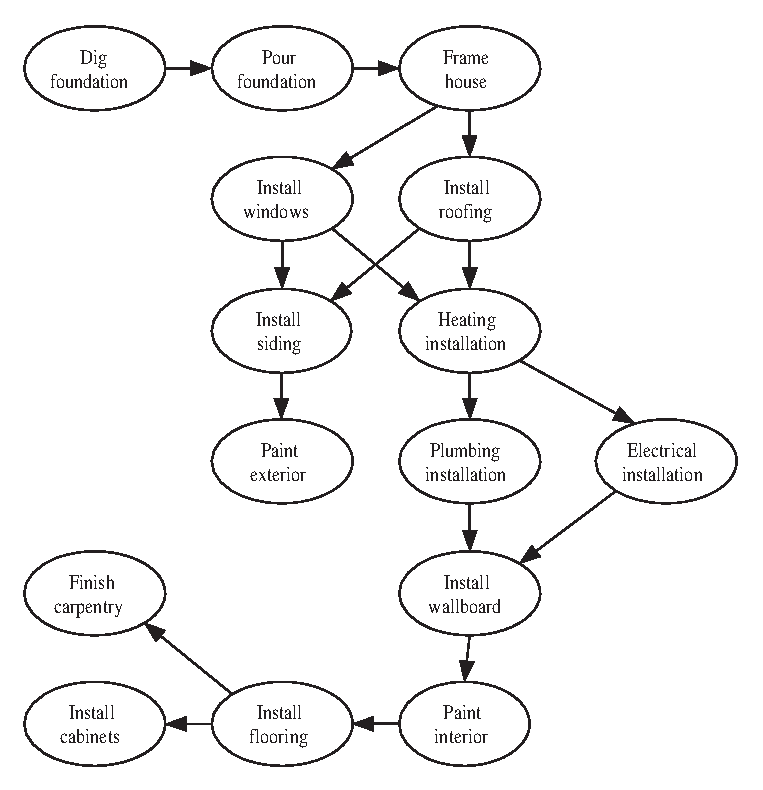
\epsfig{file=psfigures/BuildHouse.eps, width=3in}
      \end{center}
      \item Cooking and serving a spaghetti dinner
      \begin{center}
      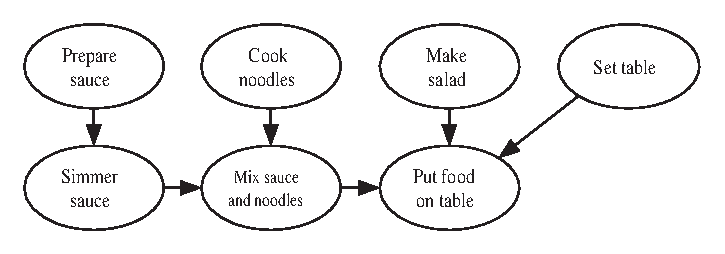
\epsfig{file=psfigures/SpaghettiDinner.eps, width=3in}
      \end{center}
      \item Cleaning an apartment
      \begin{center}
      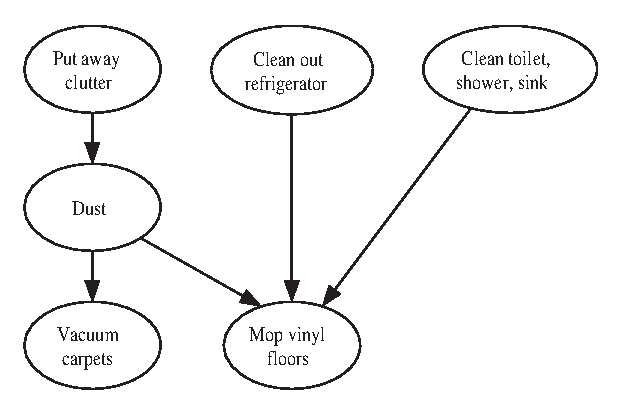
\epsfig{file=psfigures/CleanApartment.eps, width=3in}
      \end{center}
      \item Detailing an automobile
      \begin{center}
      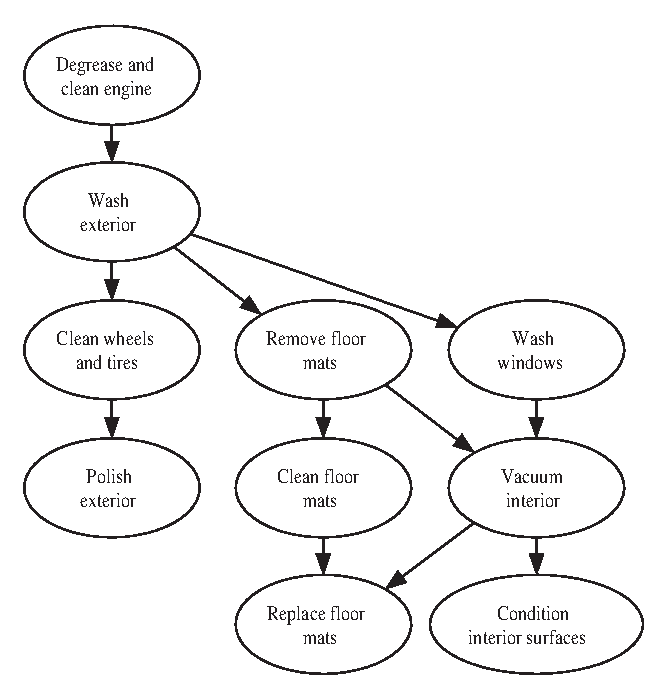
\epsfig{file=psfigures/DetailCar.eps, width=3.5in}
      \end{center}
      \end{enumerate}

\item The upper set of three nodes labeled A is a source of data parallelism.
      The lower let of three nodes labeled A is another source of data
      parallelism. B and C are functionally parallel. C and D are
      functionally parallel. D and the lower group of three nodes labeled A
      are functionally parallel.

\item The advantage of preallocation is that it reduces the overhead
      associated with assigning documents to idle processors at run-time.
      The advantage of putting documents on a list and letting processors
      remove documents as fast as they could process them is that it
      balances the work among the processors. We do not have to worry about
      one processor being done with its share of documents while another
      processor (perhaps with longer documents) still has many to process.

\item Before allocating any documents to processors we could add the lengths
      of all the documents and then use a heuristic to allocate documents to
      processors so that each processor is responsible for roughly the same
      total document length. (We need to use a heuristic, since optimally
      balancing the document lengths is an NP-hard problem.)
      This approach avoids massive imbalances in workloads. It also avoids
      run-time overhead associated with access to the shared list of
      unassigned documents.
\end{enumerate}

\chapter{Parallel Architectures}

\begin{enumerate}
\item  Hypercube networks with 2, 4, and 8 nodes. A hypercube network with
       $n$ nodes is a subgraph of a hypercube network with $2n$ nodes.
       \begin{center}
       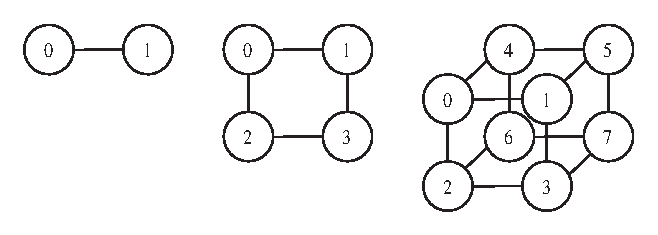
\epsfig{file=psfigures/Hypercubes.eps, width=3in}
       \end{center}

\item  A 0-dimensional hypercube can be labeled 1 way.
       A $d$-dimensional hypercube can be labeled $2^d(\log_2 d)!$ ways,
       for $d \ge 1$. Explanation: We can give any of the $2^d$ nodes the
       label 0. Once this is done, we label the neighbors of node 0.
       We have $\log_2 d$ choices for the label 1,
       $\log_2 d - 1$ choices for the label 2,
       $\log_2 d - 2$ choices for the label 4,
       $\log_2 d - 3$ choices for the label 8, etc. In other words,
       there are $(\log_2 d)!$ ways to label the nodes adjacent to node 0.
       Once this is done, all the other labels are forced.
       Hence the number of different labelings is $2^d(\log_2 d)!$.

\item  The number of nodes distance $i$ from $s$ in a $d$-dimensional
       hypercube is $d \choose i$ ($d$ choose $i$).

\item  If node $u$ is distance $i$ from node $v$ in a hypercube, exactly $i$
       bits in their addresses (node numbers) are different.
       Starting at $u$ and flipping one of these bits at a time yields the
       addresses of the nodes on a path from $u$ to $v$. Since these bits
       can be flipped in any order, there are $i!$ different paths of length
       $i$ from $u$ to $v$.

\item  If node $u$ is distance $i$ from node $v$ in a hypercube, exactly $i$
       bits in their addresses (node numbers) are different.
       Starting at $u$ and flipping one of these bits at a time yields the
       addresses of the nodes on a path from $u$ to $v$.
       To generate paths that share no intermediate vertices, we order the
       bits that are different:
       $$b_0, b_1, \ldots, b_{i-1}$$
       We generate vertices on the first path by flipping the bits
       in this order:
       $$b_0, b_1, \ldots, b_{i-1}$$
       We generate vertices on the second path by flipping the bits
       in this order:
       $$b_1, b_2, \ldots, b_{i-1}, b_0$$
       We generate vertices on the third path by flipping the bits
       in this order:
       $$b_2, b_3, \ldots, b_{i-1}, b_0, b_1$$
       This generates $i$ distinct paths from $u$ to $v$.

\item  A hypercube is a bipartite graph. Nodes whose addresses contain an
       even number of 1s are connected to nodes whose addresses contain an
       odd number of 1s. A bipartite graph cannot have a cycle of odd length.

\item  Compute the bitwise ``exclusive or'' operation on $v$ and $v$.
       The number of 1 bits in the result represents the length of the
       shortest path from $u$ to $v$. Since $u$ and $v$ have $\log n$ bits,
       there are no more than $\log n$ bits set, and
       the shortest path has length at most $\log n$.
       Number the indices from right to left, giving them values
       $0, 1, \ldots, \log n - 1$.
       Suppose the exclusive or results in $k$ bits being set, and
       these bits are at indices $b_1, b_2, \ldots, b_k$.
       This algorithm prints the shortest path from  $u$ to $v$.
       \begin{tabbing}
       \ \ \ \=\ \ \ \=\ \ \ \=\ \ \ \=\ \ \ \=\\
       $w \leftarrow u$\\
       print $w$\\
       for $i \leftarrow 1$ to $k$\\
       \> $w \leftarrow w \otimes 2^{b_k}$\quad\quad\quad$\{$exclusive or$\}$\\
       \> print $w$\\
       endfor\\
       \end{tabbing}

       Example: Find a shortest path from node 2 to node 11 in a
       four-dimensional hypercube. $0010 \otimes 1011 = 1001$.
       Hence $i_1 = 0$ and  $i_1 = 3$.  First jump:
       $0010 \otimes 0001 = 0011$. Second jump: $0011 \otimes 1000 = 1011$.
       Path is 0010 -- 0011 -- 1011.

\item  Shuffle-exchange networks with 2, 4, and 8 nodes.
       Dashed lines denote exchange links;
       solid arrows denote shuffle links.
       A shuffle-exchange network with $n$ nodes is not a subgraph of
       a shuffle-exchange network with $2n$ nodes.

       \begin{center}
       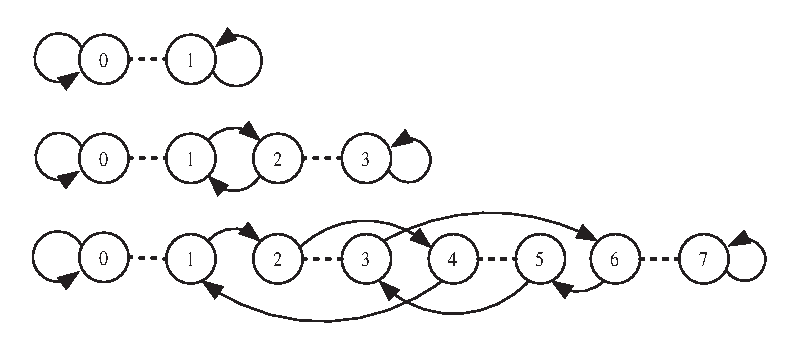
\epsfig{file=psfigures/PerfectShuffle.eps, width=4in}
       \end{center}

\item  Nodes $u$ and $v$ are exactly $2k-1$ link traversals apart if 
       one is node 0 and the other is node $2^k-1$.
       When this is the case, all $k$ bits must be changed, which means
       there must be at least $k$ traversals along exchange links.
       There must also be at least $k-1$ traversals along shuffle links
       to set up the bit reversals. The total number of link traversals
       is $2k-1$.

       In all other cases, $u$ and $v$ have at least one bit in common,
       and following no more than $k-1$ shuffle links and $k-1$ exchange
       links is sufficient to reach $v$ from $u$.

\item Algorithm to route message from $u$ to $v$ in an $n$-node
      shuffle-exchange network: 

      \begin{tabbing}
      \ \ \ \=\ \ \ \=\ \ \ \=\ \ \ \=\ \ \ \=\\
      for $i \leftarrow 1$ to $\log_2 n$ do\\
      \> $b \leftarrow u \otimes v\quad\quad \{{\rm exclusive\ or}\}$\\
      \> if $b$ is odd then\\
      \>\> print ``exchange''\\
      \> endif\\
      \> $u \leftarrow$ left\_cyclic\_rotate($u$)\\
      \> $v \leftarrow$ left\_cyclic\_rotate($v$)\\
      \> print ``shuffle''
      \end{tabbing}

      Example: Routing message from 6 to 5 in a 16-node shuffle-exchange
      network. $u = 0110$ and $v = 0101$. Algorithm produces the following
      route: exchange -- shuffle -- shuffle -- shuffle -- exchange -- shuffle.

\item \begin{enumerate}
      \item $(n/2)\log_2 n$
      \item $\log_2 n$
      \item $(n/2)\log_2 n$
      \item $4$
      \item No
      \end{enumerate}

\item Suppose the address of the destination is
      $b_{k-1}b_{k-2}\ldots b_1b_0$.
      Every switch has two edges leaving it, an ``up'' edge (toward node 0)
      and a ``down'' edge (away from node 0).
      The following algorithm indicates how to follow the edges to
      reach the destination node with the given address.

      \begin{tabbing}
      \ \ \ \=\ \ \ \=\ \ \ \=\ \ \ \=\ \ \ \=\\
      for $i \leftarrow k-1$ downto $0$ do\\
      \> if $b_i = 0$ then\\
      \>\> print ``up''\\
      \> else\\
      \>\> print ``down''\\
      \> endif\\
      endfor\\
      \end{tabbing}

\item Data parallelism means applying the same operation across a data set.
      A processor array is only capable of performing one operation at a time,
      but every processing element may perform that operation on its own
      local operands. Hence processor arrays are a good fit for 
      data-parallel programs.

\item Let $i$ be the vector length, where $1 \le i \le 50$.
      The total number of operations to be performed is $i$.
      The time required to perform these operations is
      $\lceil i/8\rceil\times 0.1\ \mu$second.
      Hence performance is
      $${{i}\over{\lceil i/8\rceil}}\times 10^7\ {\rm operations/second}$$

      For example, when vector length is 8, performance is
      80 million operations per second.
      When vector length is 50 performance is $(50/7)\times 10^7$ operations
      per second, or about 71.4 million operations per second.

\item \begin{enumerate}
      \item The efficiency is $1/k$
      \item The efficiency is
            $${\sum_{i=1}^k} I_i P_i\over{\sum_{i=1}^k I_i}$$
      \end{enumerate}

\item Large caches reduce the load on the memory bus, enabling the
      system to utilize more processors efficiently.

\item Even with large instruction and data caches, every processor still needs
      to access the memory bus occasionally. By the time the system contains
      a few dozen processors, the memory bus is typically saturated.

\item \begin{enumerate}
      \item The directory should be distributed among the multiprocessors'
            local memories so that accessing the directory does not become
            a performance bottleneck.
      \item If the contents of the directories were replicated, we would
            need to make sure the values were coherent, which is the
            problem we are trying to solve by implementing the directory.
      \end{enumerate}

\item Continuation of directory-based cache coherence protocol example.
      \begin{center}
      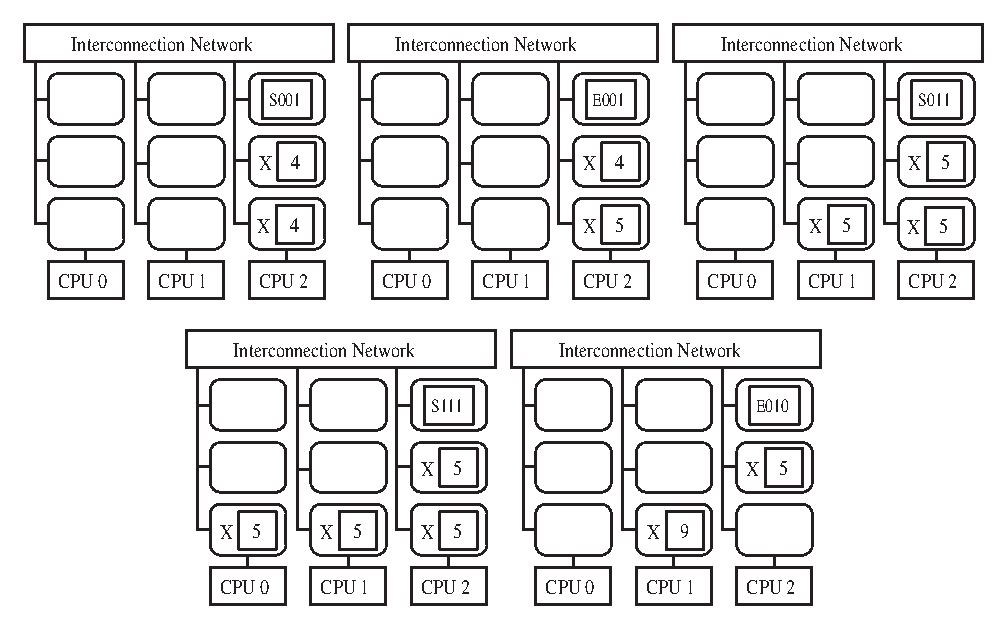
\epsfig{file=psfigures/DirectoryProtocolExample.eps, width=3.5in}
      \end{center}

\item Here is one set of examples.

      SISD: Digital Equipment Corporation PDP-11

      SIMD: MasPar MP-1

      MISD: Intel iWarp

      MIMD: Sequent Symmetry

\item Continuation of systolic priority queue example.

      \begin{center}
      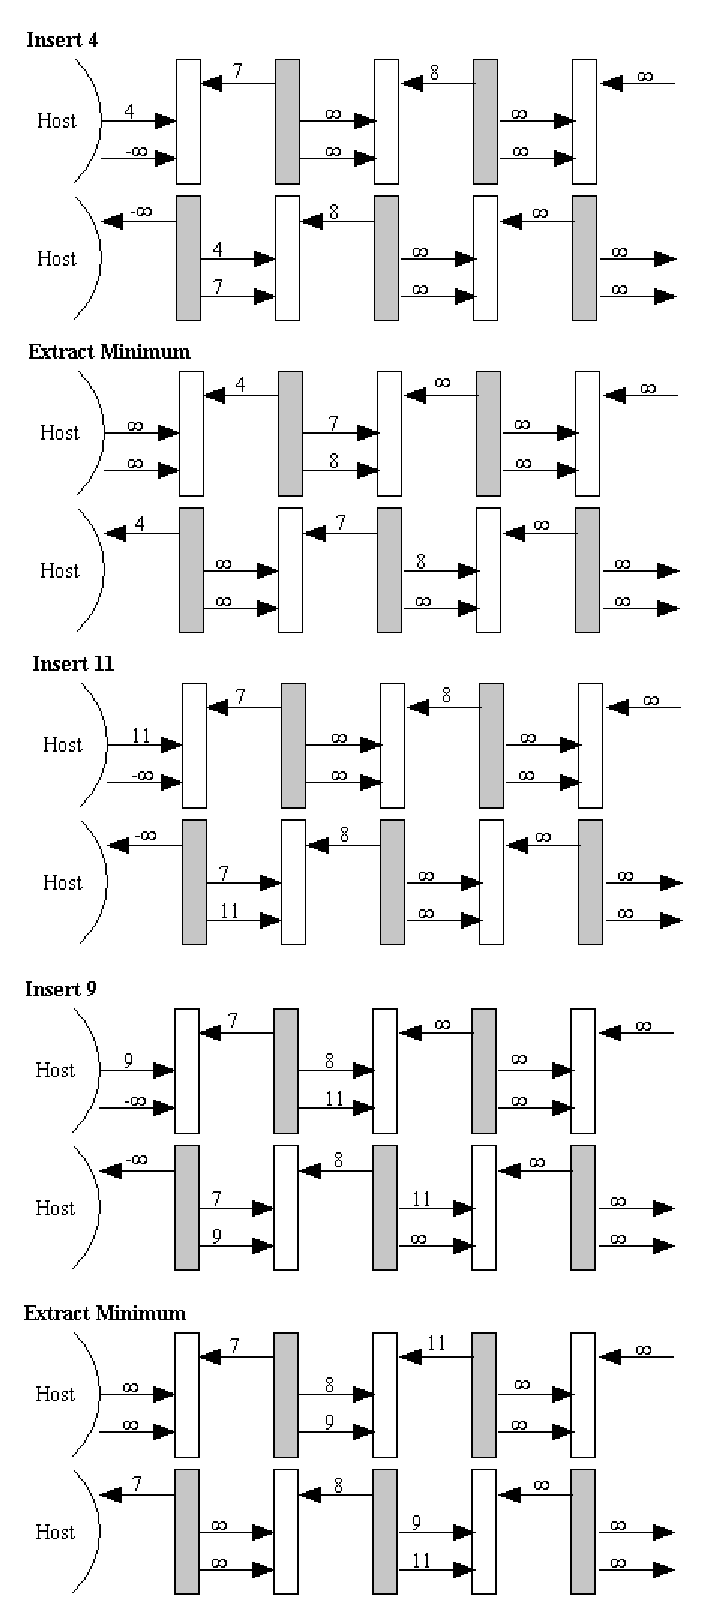
\epsfig{file=psfigures/SystolicPQ.eps, height=6.5in}
      \end{center}

\item Contemporary supercomputers must contain thousands of processors.
      Even distributed multiprocessors scale only to hundreds of processors.
      Hence supercomputers are invariably multicomputers. However, it is
      true that each node of a supercomputer is usually a multiprocessor.
      The typical contemporary supercomputer, then, is a collection of
      multiprocessors forming a multicomputer.
\end{enumerate}

\chapter{Parallel Algorithm Design}

\begin{enumerate}
\item Suppose two processors are available to find the sum of $n$ values,
      which are initially stored on a single processor.
      If one processor does all the summing, the processor utilization is
      50\%, but there is no interprocessor communication.
      If two processors share the computation, the processor utilization is
      closer to 100\%, but there is some interprocessor communication.
      One processor must send the other processor $n/2$ values and receive
      in return the sum of those values.
      The time spent in interprocessor communication prevents utilization
      from being 100\%.

\item \begin{enumerate}
      \item $\log 3 \approx 1.58$, $\lfloor\log 3\rfloor = 1$,
            $\lceil\log 3\rceil = 2$
      \item $\log 13 \approx 3.70$, $\lfloor\log 13\rfloor = 3$,
            $\lceil\log 13\rceil = 4$
      \item $\log 32 = 5$, $\lfloor\log 32\rfloor = 5$,
            $\lceil\log 32\rceil = 5$
      \item $\log 123 \approx 6.94$, $\lfloor\log 123\rfloor = 6$,
            $\lceil\log 123\rceil = 7$
      \item $\log 321 \approx 8.33$, $\lfloor\log 321\rfloor = 8$,
            $\lceil\log 321\rceil = 9$
      \end{enumerate}

\item \begin{enumerate}

      \item Binomial tree with 16 nodes

      \begin{center}
      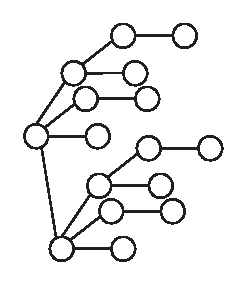
\epsfig{file=psfigures/BinomialTree16.eps, width=1.25in}
      \end{center}

      \item Binomial tree with 32 nodes

      \begin{center}
      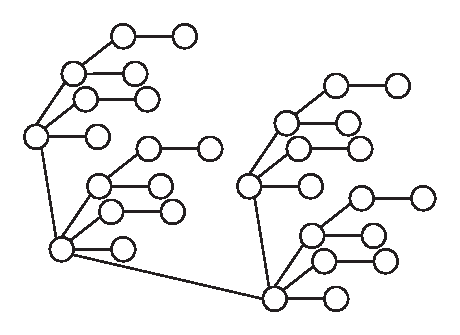
\epsfig{file=psfigures/BinomialTree32.eps, width=1.8in}
      \end{center}

      \end{enumerate}

\item \begin{enumerate}

      \item Hypercube with 16 nodes

      \begin{center}
      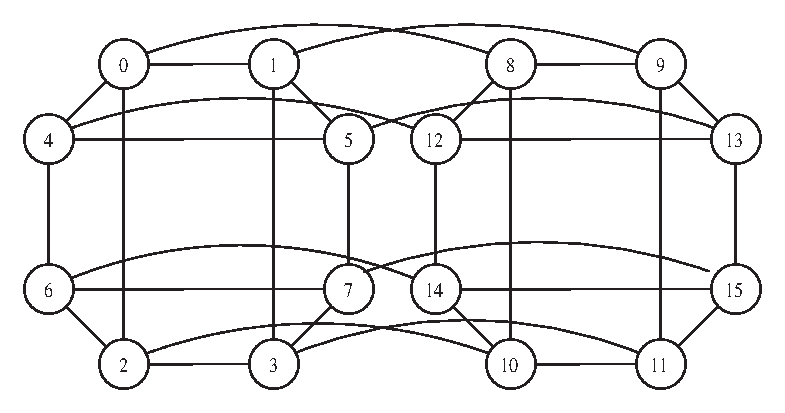
\epsfig{file=psfigures/Hypercube16.eps, width=3in}
      \end{center}

      \item Hypercube with 32 nodes

      \begin{center}
      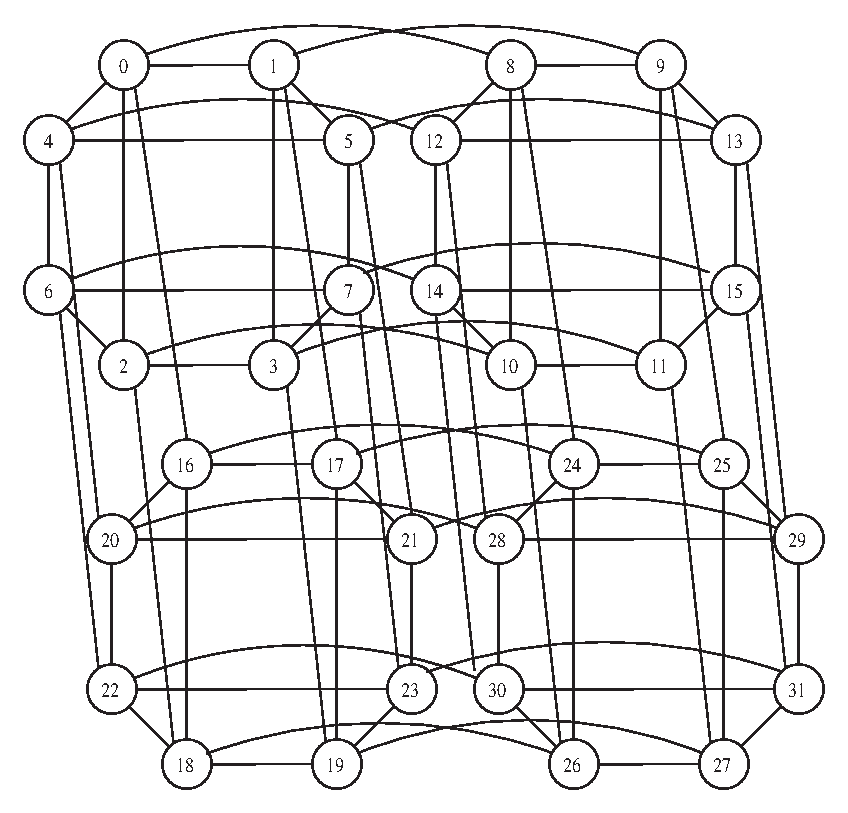
\epsfig{file=psfigures/Hypercube32.eps, width=3in}
      \end{center}

      \end{enumerate}

\item Here are four binomial trees embedded in a four-dimensional hypercube.
      All four binomial trees have the same hypercube node as their root.

      \begin{center}
      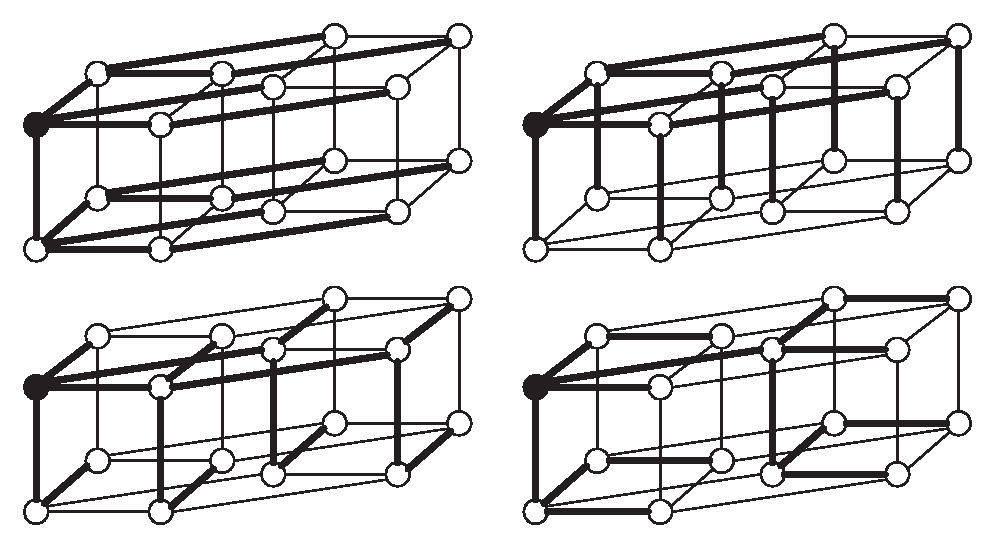
\epsfig{file=psfigures/HypercubeSubgraphs.eps, width=4in}
      \end{center}

\item Three reductions, each performed with $\lceil \log n\rceil$
      communication steps.

      \begin{center}
      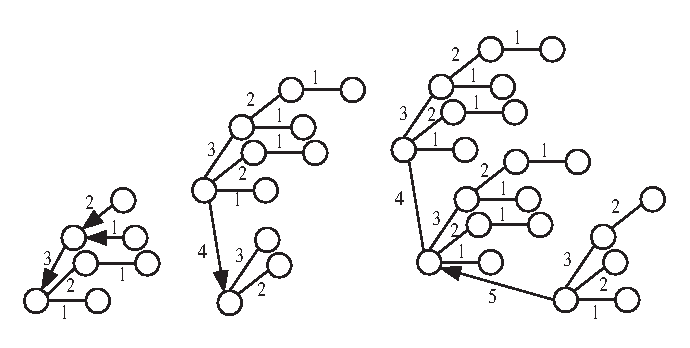
\epsfig{file=psfigures/Reductions.eps, width=4in}
      \end{center}

\item A C program that describes the communications performed by a task
      participating in a reduction.

\begin{verbatim}
int main (int argc, char *argv[])
{
   int i;
   int id;  /* Task ID */
   int p;   /* Number of tasks */
   int pow; /* ID diff between sending/receiving procs */

   if (argc != 3) {
      printf ("Command line: %s <p> <id>\n", argv[0]);
      exit (-1);
   }
   p = atoi(argv[1]);
   id = atoi(argv[2]);
   if ((id < 0) || (id >= p)) {
      printf ("Task id must be in range 0..p-1\n");
      exit (-1);
   }
   if (p == 1) {
      printf ("No messages sent or received\n");
      exit (-1);
   }
   pow = 1;
   while(2*pow < p) pow *= 2;
   while (pow > 0) {
      if ((id < pow) && (id + pow <= p))
         printf ("Message received from task %d\n",
            id + pow);
      else if (id >= pow) {
         printf ("Message sent to task %d\n", id - pow);
         break;
      }
      pow /= 2;
   }
}
\end{verbatim}

\item From the discussion in the chapter we know that we can reduce $n$ values
      in time $\Theta(\log n)$ using $n$ tasks. The only
      question, then, is whether we can improve the execution time by
      using fewer tasks.

      Suppose we use only $k$ tasks. Each task reduces about $n/k$ values,
      and then the tasks communicate to finish the reduction. The time
      complexity of this parallel algorithm would be
      $\Theta(n/k + \log k)$.
      Let's find the value of $k$ that minimizes this function.
      If $f(k) = n/k + \log k$, then
      $f'(k) = -n/k^2 + 1/k\ln{2}$.
      $f'(k) = 0$ when $k = n\ln 2$; i.e., when $k = \Theta(n)$.
      Hence the complexity of the parallel reduction is
      $\Omega(n/n + \log n) = \Omega(\log n)$.

\item Our broadcast algorithm will be based on a binomial tree communication
      pattern. Data values flow in the opposite direction they do for a
      reduction.
      \begin{enumerate}
      \item Here is a task/channel graph showing how the root task (shown in
            black) broadcasts
            to 7 other tasks in three steps. In general, use of a binomial
            tree allows a root task to broadcast to $p-1$ other tasks in
            $\lceil\log p\rceil$ communication steps.
      \begin{center}
      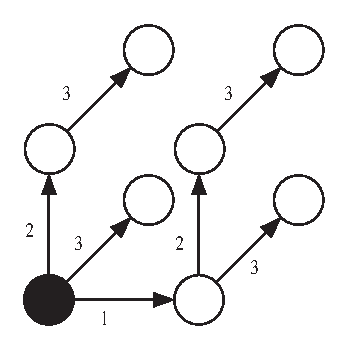
\epsfig{file=psfigures/BroadcastTaskChannel.eps, width=1.5in}
      \end{center}

      \item We prove by induction that broadcast among $p$ tasks (1 root task
            broadcasting to $p-1$ other tasks) requires at least
            $\lceil \log p\rceil$ communication steps.
            Basis. Suppose $p = 1$. No communications are needed.
            $\lceil \log 1\rceil = 0$.
            Induction. Suppose we can broadcast among $p$ tasks in
            $\lceil \log p\rceil$ communication steps, for $1 \le p \le k$.
            Then $\lceil \log k\rceil$+1 communication steps are needed to
            broadcast among $2k$ tasks, because 
            $\lceil \log k\rceil$ communication steps allow $k$ tasks to
            get the value, and 1 additional step allows each of the $k$ tasks to
            communicate the value to one of the $k$ tasks that needs it.
            $\lceil\log k\rceil + 1 = \lceil \log 2k\rceil$.
            Hence the algorithm devised in part (a) is optimal. 
      \end{enumerate}

\item The all-gather algorithm is able to route more values in the same
      because its utilization of the available communication channels is
      higher. During each step of the all-gather algorithm every task
      sends and receives a message. In the scatter algorithm the tasks
      are engaged gradually. About half of the tasks never send a message,
      and these tasks only receive a message in the last step of the
      scatter.

\item We organize the tasks into a logical
      hypercube. The algorithm has $\log p$ iterations. In the first iteration
      each task in the lower half of the hypercube swaps $p/2$ elements with
      a partner task in the upper half of the hypercube.
      After this step all elements destined for tasks in the upper half of the
      hypercube are held by tasks in the upper half of the hypercube, and
      all elements destined for tasks in the lower half of the
      hypercube are held by tasks in the lower half of the hypercube.
      At this point the algorithm is applied recursively to the lower
      and upper halves of the hypercube (dividing the hypercube into quarters).
      After $\log p$ swap steps, each process controls the correct elements.

      The following picture illustrates the algorithm for $p = 8$:

      \begin{center}
      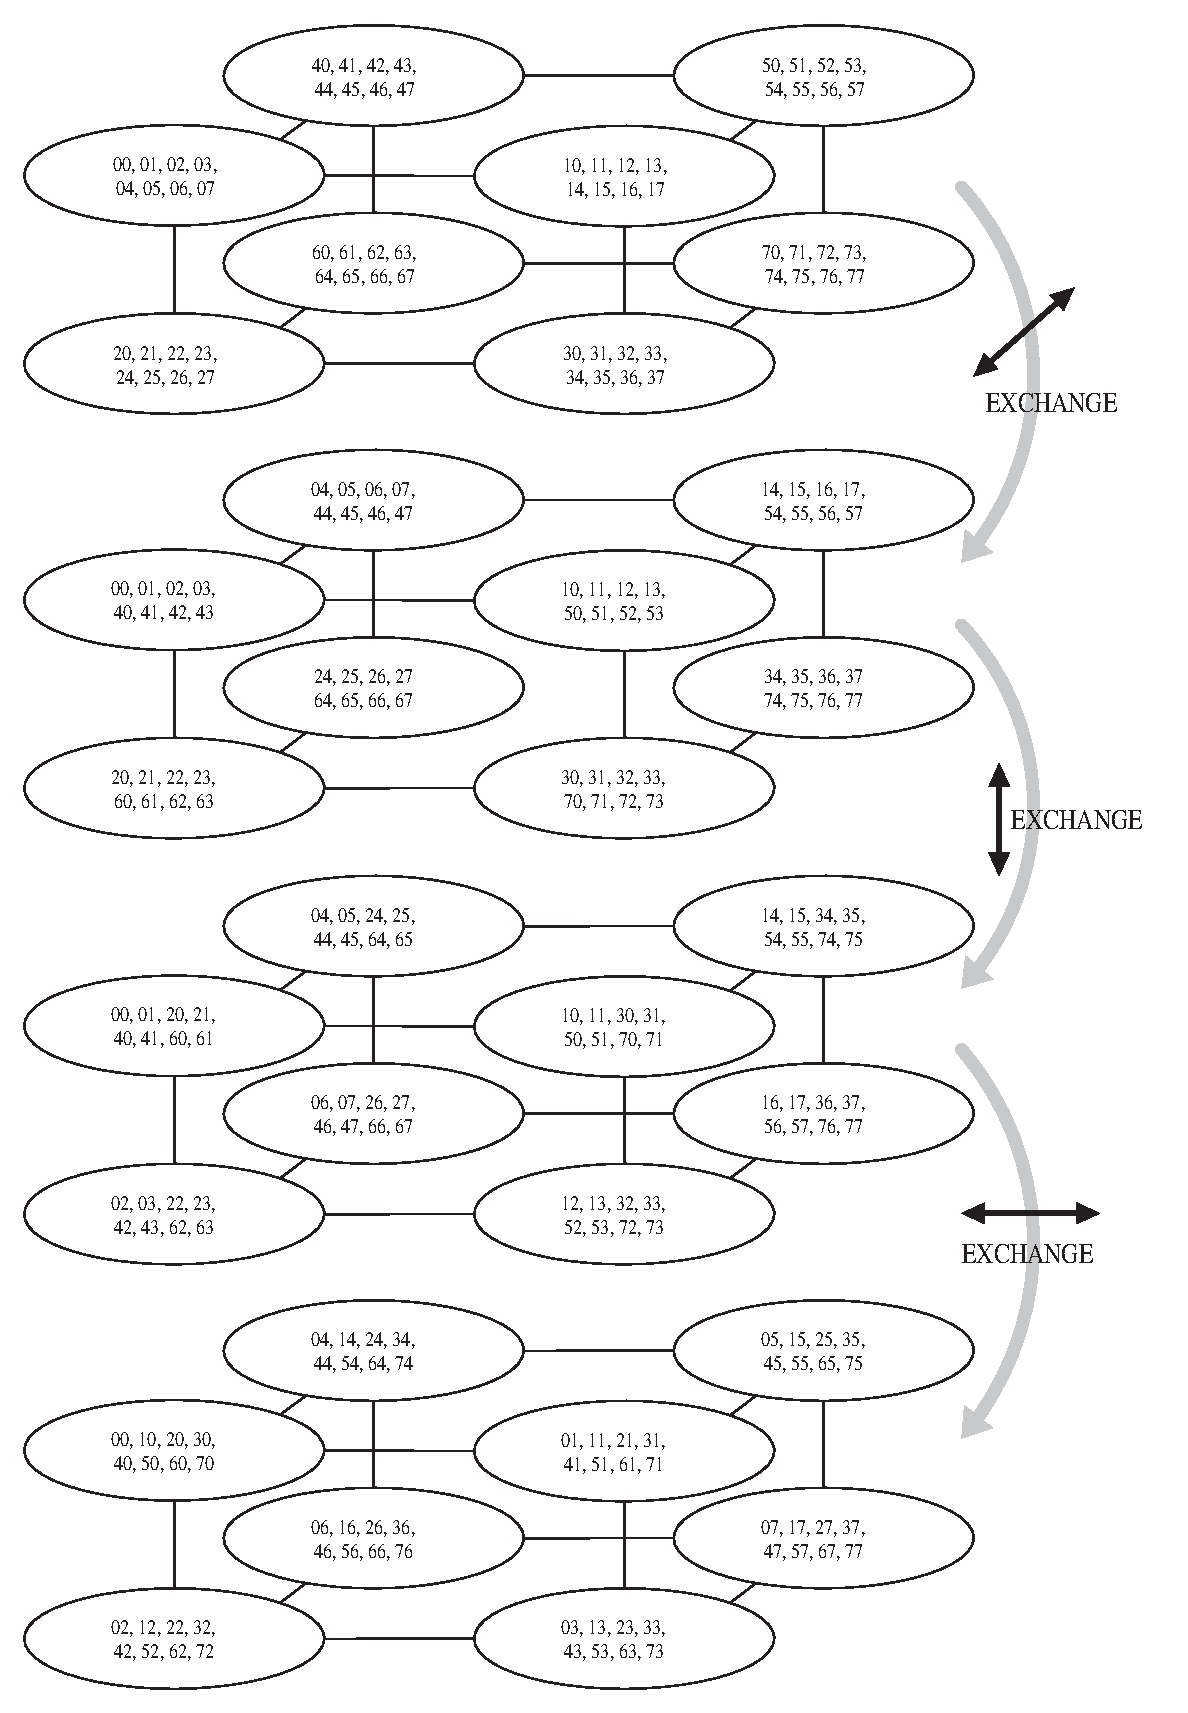
\epsfig{file=psfigures/AlltoAll.eps, width=4in}
      \end{center}
    
      During each step each process sends and receives $p/2$ elements.
      There are $\log p$ steps. Hence the complexity of the hypercube-based
      algorithm is $\Theta(p\log p)$.

\item Initially we create a primitive task for each key.
      The algorithm iterates through two steps.
      In the first step the tasks associated with even-numbered keys
      send their keys to the tasks associated with the successor keys.
      The receiving tasks keep the larger value and return the smaller value.
      In the second step the tasks associated with the odd-numbered keys
      send their keys to the tasks associated with the successor keys.
      The receiving tasks keep the larger value and return the smaller value.
      After $n/2$ iterations the list must be sorted.
      The time complexity of this algorithm is $\Theta(n)$ with $n$ 
      concurrent tasks.

      \begin{center}
      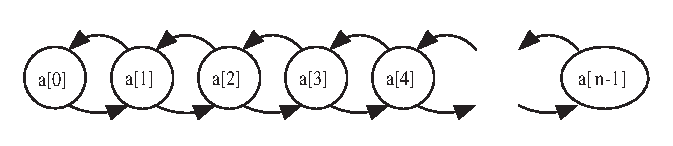
\epsfig{file=psfigures/BubbleSortPrimitive.eps, width=3.9in}
      \end{center}
    
      After agglomeration we have $p$ tasks.
      The algorithm iterates through two steps.
      In the first step each task makes a pass through its subarray, 
      from low index to high index, comparing adjacent keys. It exchanges
      keys it finds to be out of order.
      In the second step each task (except the last)
      passes its largest key to its successor task. The successor task
      compares the key it receives with it smallest key, returning the smaller
      value to the sending task.
      The computational complexity of each step is $\Theta(n/p)$.
      The communication complexity of each step is $\Theta(1)$.
      After at most $n$ iterations the list is sorted.
      The overall complexity of the parallel algorithm is $\Theta(n^2/p+n)$
      with $p$ processors.

      \begin{center}
      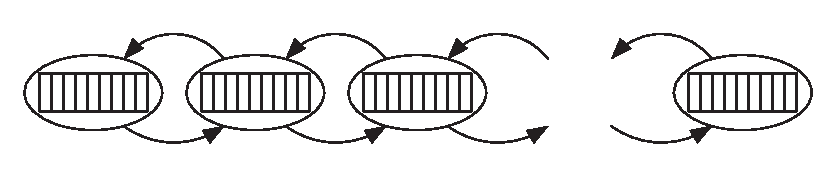
\epsfig{file=psfigures/BubbleSortAgglomerated.eps, width=3.5in}
      \end{center}

\item Initially we associate a primitive task with each pixel.
      Every primitive task communicates with tasks above it,
      below it, to its left, and to its right, if these tasks exist.
      Interior tasks have four neighbors, corner tasks has two neighbors,
      and edge tasks have three neighbors.

      \begin{center}
      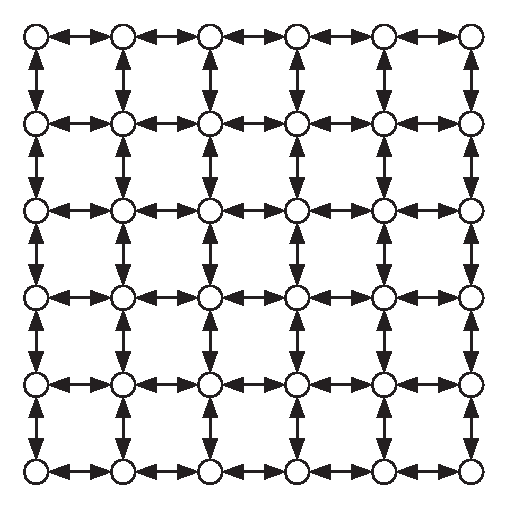
\epsfig{file=psfigures/ComponentPrimitiveTasks.eps, width=2.5in}
      \end{center}
    
      Each task associated with a 1 pixel at position $(i, j)$
      sets its component number to the unique value $n \times i + j$.
      At each step of the algorithm each task sends its current component
      number to its neighbors and receives from its neighbors their
      component numbers.
      The minimum of the component numbers received from a neighboring
      task is less than the task's current component number, then the task
      replaces its component number with this minimum value.
      In fewer than $n^2$ iterations the component numbers have stabilized.

      A good agglomeration maximizes the computation/communication ratio
      by grouping primitive tasks into rectangles that are as square as
      possible.

      \begin{center}
      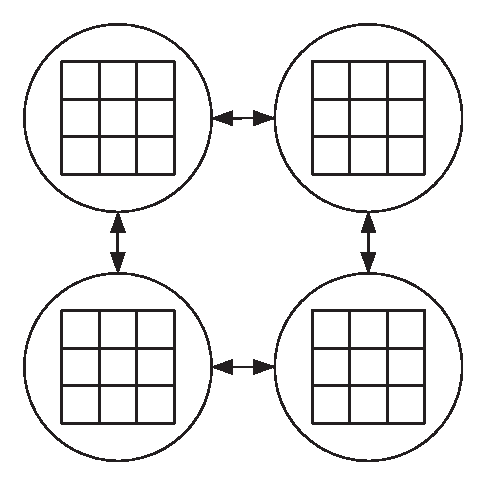
\epsfig{file=psfigures/ComponentAgglomerated.eps, width=2in}
      \end{center}

\item We set up one ``manager'' task and a bunch of ``worker'' tasks.
      A pair of channels connects the manager with each worker.
      All tasks have a copy of the dictionary.

      \begin{center}
      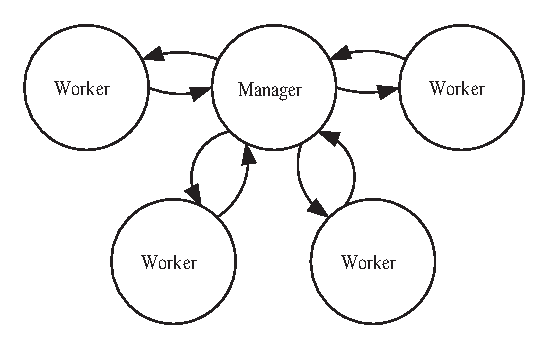
\epsfig{file=psfigures/ManagerWorker.eps, width=3in}
      \end{center}

      The manager partially fills out a crossword puzzle and then assigns
      it to a worker to complete. By assigning partially-completed puzzles
      to the workers, the manager ensures no two workers are doing the same
      thing. A worker sends a message back to the manager either when it has
      successfully filled in a puzzle or when it has determined there is no 
      way to solve the partially filled-in puzzle it received.
      When the manager receives a solved puzzle from a worker it tells all
      the workers to stop.

\item Each primitive task is responsible for the coordinates of one of the
      houses. All primitive tasks have the coordinates of the train station.
      Each task computes the euclidean distance from its house to the train
      station.
      Each task $i$ contributes a pair $(d_i, i)$ to a reduction in which
      the operation is minimum. The result of the reduction is the pair
      $(d_k, k)$, where $d_k$ is the minimum of all the submitted values
      of $d_i$, and $k$ is the index of the task submitting $d_k$.
      The communication pattern is a binomial tree, allowing the reduction
      to take place in logarithmic time.
      A sensible agglomeration assigns about $n/p$ coordinate pairs to each 
      of $p$ tasks. Each task find the closest house among the $n/p$ houses
      it has been assigned, then participates in the reduction step with the
      other tasks.

      The ``before'' and ``after'' task/channel graphs should resemble
      Figure 3.16.

\item The text is divided into $p$ segments, one per task.
      Each task is responsible for searching its portion of the text for the
      pattern.
      We need to be able to handle the case where the pattern is split between
      two tasks' sections.
      Suppose the pattern has $k$ letters.
      Each of the first $p-1$ tasks must pass the last $k-1$ letters of its
      portion of the text to the subsequent task.
      Now all occurrences of the pattern can be detected.

      After the tasks have completed their portions of the search, a
      gather communication brings together information about all occurrences
      of the pattern.

      In the following task/channel graph, the straight arrows represent
      channels used to copy the last final $k-1$ letters of each task's
      section to its successor task. The curved arrows represent channels
      used for the gather step.

      \begin{center}
      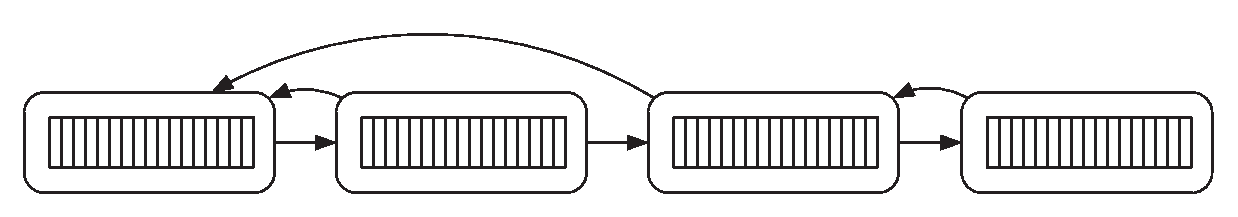
\epsfig{file=psfigures/StringMatching.eps, width=4in}
      \end{center}

\item If the pattern is likely to appear multiple times in the text, and if
      we are only interested in finding the first occurrence of the pattern
      in the text, then the allocation of contiguous blocks of text to
      the tasks is probably unacceptable.
      It makes it too likely that the first task will find the pattern,
      making the work of the other tasks superfluous. A better strategy is to
      divide the text into $jp$ portions and allocate these portions in an
      interleaved fashion to the tasks. Each task ends up with $j$ segments
      from different parts of the text.

      \begin{center}
      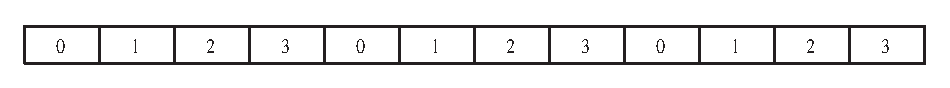
\epsfig{file=psfigures/PatternMatchCyclic.eps, width=4in}
      \end{center}

      As before, the final $k-1$ letters in each segment must be copied into
      the successor segment, in case the pattern is split across two segments.

      Communication tasks enable one task
      to inform the other tasks as soon as it has found a match.

\item Associate a primitive task with each key.
      In the first step the tasks perform a max-reduction on the keys.
      In the second step the maximum key is broadcast to the tasks.
      In the third step each task compares its key with the maximum.
      In the fourth step the tasks perform another max-reduction.
      Every task submits a candidate key to the second max-reduction
      except the task whose key is equal to the maximum key.

      We can reduce the communication complexity of the parallel algorithm
      without increasing the computation time on $p$ processors by
      agglomerating groups of $n/p$ primitive tasks into larger tasks.

\item This solution is similar to the previous solution, except that in
      the max-reduction step each task submits the pair $(k_i, i)$,
      where $k_i$ is the value of the key and $i$ is its index in the list.
      The result of the max-reduction is the pair $(m_i, i)$, where $m_i$
      is the smallest key submitted and $i$ is its list position.
      This pair is broadcast to all the primitive tasks.
      In the fourth step the tasks perform another max-reduction.
      Every task submits a candidate key except the task whose index is equal
      to the index received in the broadcast step.
      
      We can reduce the communication complexity of the parallel algorithm
      without increasing the computation time on $p$ processors by
      agglomerating groups of $n/p$ primitive tasks into larger tasks.

\end{enumerate}

\chapter{Message-passing Programming}

\begin{enumerate}
\item \begin{enumerate}
      \item Give the pieces of work the numbers $0, 1, 2, \ldots, n-1$.
            Process $k$ gets the pieces of work $k, k + p, k + 2p,$ etc.,
      \item Piece of work $j$ is handled by process $j \bmod p$.
      \item $\lceil n/p\rceil$
      \item If $n$ is an integer multiple of $p$, then all processes have
            the same amount of work. Otherwise, $n \bmod p$ processes have
            more pieces of work---$\lceil n/p\rceil$. These are
            processes $0, 1, \ldots, (n \bmod p)-1$.
      \item $\lfloor n/p\rfloor$
      \item If $n$ is an integer multiple of $p$, then all processes have
            the same amount of work. Otherwise, $p - (n \bmod p)$ processes have
            less pieces of work---$\lfloor n/p\rfloor$. These are
            processes $(n \bmod p), (n \bmod p)+1, \ldots, p-1$.
      \end{enumerate}

\item \begin{enumerate}
      \item 241
      \item Overflow. In C, get 128 as result.
      \item 99
      \item 13
      \item 127
      \item 0
      \item 1
      \item 1
      \end{enumerate}

\item Modified version of function {\tt check\_circuit}.

\begin{verbatim}
int check_circuit (int id, int z) {
   int v[16];        /* Each element is a bit of z */
   int i;

   for (i = 0; i < 16; i++) v[i] = EXTRACT_BIT(z,i);
   if ((v[0]||v[1]) && (!v[1]||!v[3]) && (v[2]||v[3])
      && (!v[3] || !v[4]) && (v[4] || !v[5])
      && (v[5] || !v[6]) && (v[5] || v[6])
      && (v[6] || !v[15]) && (v[7] || !v[8])
      && (!v[7] || !v[13]) && (v[8] || v[9])
      && (v[8] || !v[9]) && (!v[9] || !v[10])
      && (v[9] || v[11]) && (v[10] || v[11])
      && (v[12] || v[13]) && (v[13] || !v[14])
      && (v[14] || v[15])) {
      printf ("%d) %d%d%d%d%d%d%d%d%d%d%d%d%d%d%d%d\n",
         id,v[0],v[1],v[2],v[3],v[4],v[5],v[6],v[7],
         v[8],v[9],v[10],v[11],v[12],v[13],v[14],v[15]);
      fflush (stdout);
      return 1;
   } else return 0;
}
\end{verbatim}

\item See Figure 4.6.

\item \begin{enumerate}
      \item The circuit can be represented by a logical expression using
            the same syntax as the C programming language. Parentheses
            are used as necessary to indicate the order in which
            operators should be applied.
      \item Creating a syntax-free grammar for logical expressions is easy.
            We could write a top-down or a bottom-up parser to construct a
            syntax tree for the circuit.
      \item The circuit would be represented by an expression tree. The
            leaves of the tree would be the inputs to the circuit. The
            interior nodes of the tree would be the logical gates. A $not$
            gate would have one child; $and$ and $or$ gates would have
            two children.
      \end{enumerate}

\vfill\eject
\item  Parallel variant of Kernighan and Ritchie's ``hello, world'' program.

\begin{verbatim}
#include "mpi.h"
#include <stdio.h>

int main (int argc, char *argv[]) {
   int id;               /* Process rank */

   MPI_Init (&argc, &argv);
   MPI_Comm_rank (MPI_COMM_WORLD, &id);

   printf ("hello, world, from process %d\n", id);
   fflush (stdout);
   MPI_Finalize();
   return 0;
}
\end{verbatim}

\end{enumerate}

\chapter{The Sieve of Eratosthenes}

\begin{enumerate}
\item \begin{enumerate}
      \item The first $p-1$ processes get $\lceil n/p \rceil$ elements and the
            last process does not get any elements when $n = k(p-1)$,
            where $k$ is an integer greater than 1 and less than $p$.
            Here are the cases where this happens for $n \le 10$:
            $n = 4$ and $p = 3$;
            $n = 6$ and $p = 4$;
            $n = 8$ and $p = 5$;
            $n = 9$ and $p = 4$; and
            $n = 10$ and $p = 6$.
      \item In order for $\lfloor p/2 \rfloor$ processes to get no values,
            $p$ must be odd and $n$ must be equal to $p+1$. Here are the
            cases where this happens for $n \le 10$:
            $n = 4$ and $p = 3$;
            $n = 6$ and $p = 5$;
            $n = 8$ and $p = 7$; and
            $n = 10$ and $p = 9$.
      \end{enumerate}

\item We list the number of elements held by each process for each scheme.
      For example, (4, 3, 3) means that the first process has four elements
      and the second and third processes have three elements each.
      \begin{enumerate}
      \item Scheme 1: (4, 4, 4, 3); Scheme 2: (3, 4, 4, 4)
      \item Scheme 1: (3, 3, 3, 2, 2, 2); Scheme 2: (2, 3, 2, 3, 2, 3)
      \item Scheme 1: (4, 3, 3, 3, 3); Scheme 2: (3, 3, 3, 3, 4)
      \item Scheme 1: (5, 5, 4, 4); Scheme 2: (4, 5, 4, 5)
      \item Scheme 1: (4, 4, 3, 3, 3, 3); Scheme 2: (3, 3, 4, 3, 3, 4)
      \item Scheme 1: (4, 4, 3, 3, 3, 3, 3); Scheme 2: (3, 3, 3, 4, 3, 3, 4)
      \end{enumerate}

\item This table shows the predicted execution time of the first
      parallel implementation of the Sieve of Eratosthenes on 1--16
      processors.

\begin{tabular}{|c|c|}
\hline
{\it Processors}&{\it Time} \\
\hline
1 & 24.910 \\
2 & 12.727 \\
3 & 8.846  \\
4 & 6.770 \\
5 & 5.796 \\
6 & 4.966 \\
7 & 4.373 \\
8 & 3.928 \\
9 & 3.854 \\
10 & 3.577 \\
11 & 3.350 \\
12 & 3.162 \\
13 & 3.002 \\
14 & 2.865 \\
15 & 2.746 \\
16 & 2.643 \\
\hline
\end{tabular}
            
\item This table compares the predicted versus actual execution time of
      the second parallel implementation of the Sieve of Eratosthenes on
      a commodity cluster.

\begin{tabular}{|c|c|c|c|}
\hline
{\it Processors}&{\it Predicted Time} & {\it Actual Time} & {\it Error (\%)}\\
\hline
1 & 12.455 & 12.237 & 1.78\\
2 & 6.499 &  6.609  & 1.66\\
3 & 4.695 &  5.019  & 6.46\\
4 & 3.657 &  4.072  & 10.19\\
5 & 3.305 &  3.652  & 9.50\\
6 & 2.890 &  3.270  & 11.62\\
7 & 2.594 &  3.059  & 15.20\\
8 & 2.371 &  2.856  & 16.98\\
\hline
\end{tabular}

The average error in the predictions for 2--7 processors is 10.23\%.

\vfill\eject

\item This table compares the predicted versus actual execution time of
      the third parallel implementation of the Sieve of Eratosthenes on
      a commodity cluster.

\begin{tabular}{|c|c|c|c|}
\hline
{\it Processors}&{\it Predicted Time} & {\it Actual Time} & {\it Error (\%)}\\
\hline
1 & 12.457 & 12.466 & 0.07\\
2 & 6.230 &  6.378  & 2.32\\
3 & 4.154 &  4.272  & 2.76\\
4 & 3.116 &  3.201  & 2.66\\
5 & 2.494 &  2.559  & 2.54\\
6 & 2.078 &  2.127  & 2.30\\
7 & 1.782 &  1.820  & 2.09\\
8 & 1.560 &  1.585  & 1.58\\
\hline
\end{tabular}

The average error in the predictions for 2--7 processors is 2.32\%.

%Exercise 5-6
\addtocounter{enumi}{1}
%Exercise 5-7
\addtocounter{enumi}{1}
%Exercise 5-8
\addtocounter{enumi}{1}
%Exercise 5-9
\addtocounter{enumi}{1}

\item The first disadvantage is a lack of scalability.
      Since every process must set aside storage representing the integers
      from 2 through $n$, the maximum value of $n$ cannot increase when
      $p$ increases. The second disadvantage is that the OR-reduction step
      reduces extremely large arrays. Communicating these arrays among the
      processors will require a significant amount of time. The third
      disadvantage is that the workloads among the processors are
      unbalanced. For example, in the case of three processors, the processor
      sieiving with 2, 7, 17, etc. will take significantly to mark multiples
      of its primes than the processor sieving with 5, 13, 23, etc.

\end{enumerate}

\chapter{Floyd's Algorithm}

\begin{enumerate}
\item Suppose $n = kp + r$, where $k$ and $r$ are nonnegative integers and
      $0 \le r < p$. Note that this implies $k = \lceil n/p\rceil$.

      If $r$ (the remainder) is 0, then all processes are
      assigned $n/p = \lceil n/p\rceil$ elements. Hence the last process is
      responsible for $\lceil n/p \rceil$ elements.

      If $r > 0$, then the last process is responsible for elements
      $\lfloor(p-1)n/p\rfloor$ through $n-1$.

\begin{equation*}
\begin{split}
\lfloor(p-1)n/p\rfloor &= \lfloor(p-1)(kp+r)/p\rfloor \\
                       &= \lfloor p(kp+r)/p - kp/p -r/p\rfloor \\
                       &= (kp + r) - k - \lfloor r/p\rfloor \\
                       &= kp + r - k - 1 \\
                       &= n - (k + 1)\\
\end{split}
\end{equation*}

      The total number of elements the last process is responsible for is
      $$(n - 1) - (n - (k+1)) + 1= k + 1 = \lceil n/p \rceil$$

\item Process 0 only needs to allocate $\lfloor n/p\rfloor$ elements to
      store its portion of the file.
      Since it may need to input and pass along
      $\lceil n/p\rceil$ elements to some of the processes, process 0 cannot
      use its file storage buffer as a temporary buffer holding the elements
      being passed along to the other processes. (Room for one extra element
      must be allocated.) In contrast, process 3 will eventually be responsible
      for $\lceil n/p\rceil$ elements of the file.
      Since no process stores more elements, the space allocated for
      process 3's portion of the file is sufficient to be used as a temporary
      message buffer.

      We see this played out in Figure 6.6, in which process 0 is responsible
      for $\lfloor 14/4\rfloor = 3$ elements, while process 3 is responsible
      for $\lceil 14/4\rceil = 4$ elements.

\item We need to consider both I/O and communications within Floyd's algorithm
      itself.
      File input will be more complicated, assuming the distance matrix
      is stored in the file in row-major order.
      One process is responsible for accessing the file.
      It reads in one row of the matrix at a time and then
      scatters the row among all the processes.
      After $n$ read-and-scatter steps, each process has its portion of
      the distance matrix.

      During iteration $k$ of Floyd's algorithm,
      the process controlling column $k$ must
      broadcast this column to the other processes.
      No other communications are needed to perform the computation.

      In order to print the matrix, one process should be responsible for
      all of the printing. Each row is gathered onto the one process
      that prints the row before moving on to print the next row.

\item Several changes are needed when switching from a rowwise block
      striped decomposition to a rowwise interleaved striped decomposition.

      First, the process that inputs the matrix from the file can only
      read one row at a time. In each of $n$ iterations, the process reads
      row $i$ and sends it to process $i \bmod p$ (except when it keeps rows
      it is responsible for).
      Hence this decomposition results in more messages being sent by the
      process responsible for reading the matrix from the file.

      Second, in the
      performance of Floyd's algorithm, the computation of the process
      broadcasting row $k$ is different. 
      In the block decomposition the process controlling row $k$ is
      $\lfloor p(k+1)-1)/n\rfloor$.
      In the interleaved decomposition the process controlling row $k$ is
      $k \bmod p$.

      Third, when the matrix is printed, processes send their rows to
      the printing process one at a time, instead of all at once.
      The printing process must print the first row held by process 0,
      the first row held by process 1, $\ldots$, the first row held by process
      $p-1$, the second row held by process 0, etc.
      Hence this decomposition results in more messages being received by
      the process responsible for printing the matrix.

\item \begin{enumerate}
      \item The processes are logically organized into a square mesh.
            During each iteration of the outer loop of the algorithm,
            a process needs access to {\tt a[i][k]} and {\tt a[k][j]} in order
            to update {\tt a[i][j]}.
            Hence every process controlling a portion of row {\tt k} must
            broadcast it to other processes in the same column of the process
            mesh.  Similarly, every process controlling a portion of
            column {\tt k} must broadcast it to other processes in the same
            row of the process mesh.

            \begin{center}
            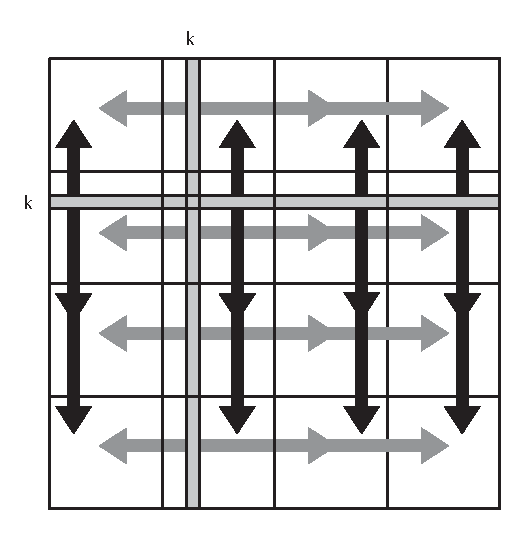
\epsfig{file=psfigures/FloydBlockCommunication.eps, width=3in}
            \end{center}

            Note that the $\sqrt{p}$ broadcasts across rows of the process
            mesh may take place simultaneously.
            The $\sqrt{p}$ broadcasts across columns of the process
            mesh may also take place simultaneously.

      \item During each iteration there is are two broadcast phases.
            The communication time is the same for both phases.
            A total of $n/\sqrt{p}$ data items, each of length 4 bytes,
            are broadcast among a group of $\sqrt{p}$ processes.
            The time needed for the broadcast is
            $$\lceil\log\sqrt{p}\rceil(\lambda + 4n/{(\sqrt{p}\beta)}$$
            Since there are two broadcast phases per iteration and $n$
            iterations, the total communication time is
            $$2n\lceil\log\sqrt{p}\rceil(\lambda + 4n/{(\sqrt{p}\beta)})$$
      \item Since $2n\lceil\log\sqrt{p}\rceil = n\lceil\log p\rceil$,
            the number of messages sent by both algorithms is the same.
            However, the parallel version of Floyd's algorithm that assigns
            each process a square block of the elements of {\bf A} has its
            message transmission time reduced by a factor of $\sqrt{p}$.
            Hence it is superior.
      \end{enumerate}

\item We need to compute
      $$n^2\lceil n/p\rceil\chi + n\lceil\log p\rceil(lambda + 4n/\beta)$$
      where $n = 1000$, $p = 16$, $\chi = 25.5$ nanosec,
      $\lambda = 250\ \mu$sec, and $\beta = 10^7$ bytes/sec.
      The result is 4.19 seconds.

\item This table predicts the execution times (in seconds)
      when executing Floyd's algorithm on problems of
      size 500 and 2,000 with $1, 2, \ldots, 8$ processors.
      The computer has the same values of $\chi$, $\lambda$, and
      $\beta$ as the system used for benchmarking in this chapter.
      \vskip\baselineskip
      
\begin{tabular}{|c|c|c|}
\hline
{\it Processors}&$n = 500$ & $n = 2000$ \\
\hline
1 & 3.19 & 204.0 \\
2 & 1.72 & 102.5 \\
3 & 1.32 & 69.0 \\
4 & 1.05 & 52.0 \\
5 & 1.01 & 42.3 \\
6 & 0.91 & 35.6 \\
7 & 0.83 & 30.7 \\
8 & 0.78 & 27.0 \\
\hline
\end{tabular}
\end{enumerate}

\chapter{Performance Analysis}

\begin{enumerate}
\item
The speedup formula is
$$\psi(n,p) \le
{{\sigma(n) + \varphi(n)}\over{\sigma(n) + \varphi(n)/p + \kappa(n,p)}}$$
We want to find $p_0$ such that $p > p_0 \Rightarrow \psi(n,p) < \psi(n,p_0)$.
From the formula we see this is the same as saying
we want to find $p_0$ such that
$p > p_0 \Rightarrow \varphi(n)/p + \kappa(n,p) >
                              \varphi(n)/p_0 + \kappa(n,p_0)$.
We are told that $\kappa(n,p) = c\log p$.
Let
$$f(p) = \varphi(n)/p + c\log p$$
Then
$$f'(p) = -\varphi(n)/p^2 + c/(p\ln 2)$$
Finding the point where the slope is 0:
$$f'(p) = 0 \Rightarrow p = \varphi(n)\ln{2}/c$$
Let
$$p_0 = \lceil\varphi(n)\ln{2}/c\rceil$$
Since $f'(p) > 0$ when $p > p_0$, $f(p)$ is increasing for $p > p_0$.
Therefore, there exists a $p_0$ such that $p > p_0 \Rightarrow
\psi(n,p) < \psi(n,p_0)$.

\item
The definition of efficiency is
$$\varepsilon \le
{{\sigma(n) + \varphi(n)}\over{p\sigma(n) + \varphi(n) + p\kappa(n,p)}}$$
Since $p\sigma(n)$ and $\kappa(n,p)$ are both nondecreasing functions of
$p$, the denominator is a nondecreasing function of $p$, meaning that
$\varepsilon(n,p)$ is a nonincreasing function of $p$.
Hence $p' > p \Rightarrow \varepsilon(n,p') \le \varepsilon(n,p)$.

\item Sequential execution time is 0.01 seconds.
Speedup is parallel execution time divided by sequential execution time.

\begin{tabular}{|c|c|}
\hline
{\it Processors}&{\it Speedup}\\
\hline
1 & 1.00 \\
2 & 1.96 \\
3 & 2.83 \\
4 & 3.70 \\
5 & 4.35 \\
6 & 5.08 \\
7 & 5.79 \\
8 & 6.45 \\
9 & 6.62 \\
10 & 7.14 \\
11 & 7.64 \\
12 & 8.11 \\
13 & 8.55 \\
14 & 8.97 \\
15 & 9.37 \\
16 & 9.76 \\
\hline
\end{tabular}

\item By Amdahl's Law,
$$\psi \le {{1}\over{f + (1-f)/p}} = {{1}\over{0.05 + 0.95/10}} = 6.90$$
Maximum achievable speedup is 6.90.

\item Using Amdahl's Law,
$$10 \le {{1}\over{0.06 + .94/p}} \Rightarrow p \ge 24$$
Hence at least 24 processors are needed to achieve a speedup of 10.

\item Starting with Amdahl's Law:
$$\psi \le {{1}\over{f + (1-f)/p}}$$
we take the limit as $p \rightarrow \infty$ and find that
$$\psi \le {{1}\over{f}} \Rightarrow f \le {{1}\over{\psi}}$$
In order to achieve a speedup of 50, no more than 1/50th (2\%) of a program's
execution time can be spent in inherently sequential operations.

\item We begin with Amdahl's Law and solve for $f$:
\begin{equation*}
\begin{split}
            & \psi \le {{1}\over{f + (1-f)/p}} \\
\Rightarrow & 9 \le {{1}\over{f + (1-f)/10}} \\
\Rightarrow & 9 \le {{1}\over{f + 0.1 - 0.1f}} \\
\Rightarrow & 9f + 0.9 -0.9f \le 1 \\
\Rightarrow & 8.1f \le 0.1\\
\Rightarrow & f \le 0.0123
\end{split}
\end{equation*}
At most 1.23\% of the computations performed by the program are
inherently sequential.

\item Gustafson-Barsis's Law states that
$$\psi \le p + (1-p)s$$
In this case $s = 9/242 = 0.037$.
Hence the scaled speedup on 16 processors is $16 + (1-16)0.0372 = 15.4$.

\item By Gustafson-Barsis's Law, scaled speedup is $40 + (1-40)0.01 = 39.6$.

\item This problem asks us to apply the Karp-Flatt metric.
      \renewcommand{\theenumii}{\Roman{enumii}}
      \begin{enumerate}
      \item The answer is (B). The experimentally determined serial fraction
            is 0.2 for $2 \le p \le 8$. If it remains at 0.2,
            speedup on 16 processors will 4, only 20\% higher
            than on 8 processors.
      \item The answer is (C). The experimentally determined serial fraction
            is growing linearly with $p$. If it continues to increase at this
            rate, speedup on 16 processors will be 4,
            which is 8\% lower than on 8 processors.
      \item The answer is (A). The experimentally determined
            serial fraction is holding steady at 0.06.
            If it remains at 0.06, speedup on 16 processors will be 8.42,
            or 49\% higher than on 8 processors.
      \item The answer is (A). The experimentally determined
            serial fraction is growing logarithmically
            with $p$. If it has the value 0.05 when $p = 16$, speedup will be
            9.14, or 46\% higher than on 8 processors.
      \item The answer is (B). The experimentally determined serial fraction
            is growing very slowly, but it is quite large.
      \item The answer is (A). The experimentally determined serial fraction
            is small and growing slowly.
      \end{enumerate}

\item In Amdahl's Law, when you fix $f$ and increase $p$, the problem size
      does not change. This is because the focus of Amdahl's Law is on the
      effects of applying more processors to a particular problem.
      Hence as $p \rightarrow \infty$, the maximum speedup converges on $1/f$.

      In contrast, with Gustafson-Barsis' Law, when you fix $s$ and increase
      $p$, the proportion of inherently sequential operations actually drops.
      For example, suppose $s = 0.1$ and $p = 2$. 
      Then two processors are busy 90\% of the time and one processor is busy
      10\% of the time.
      The number of inherently sequential operations represents just over
      5\% of the total computation.
      In contrast, suppose $s = 0.1$ and $p = 20$.
      Now twenty processors are busy 90\% of the time and one processor is
      busy 10\% of the time.
      The number of inherently sequential operations represents just over
      $0.5\%$ of the total computation.

      Because the proportion of inherently sequential operations drops
      when fixing $s$ and increasing $p$, the scaled speedup predicted by
      Gustafson-Barsis' Law increases without bound.

\item Here are three reasons why it may be impossible to
      solve the problem within
      a specified time limit, even if you have access to al the processors
      you care to use.

      First, the problem may not be amenable to a parallel
      solution.

      Second, even if the bulk of the problem can be solved by a parallel
      algorithm, there may be a sequential component (such as file I/O) that
      limits the speedup achievable through parallelism.

      Third, even if there is no significant sequential component,
      interprocessor communication overhead may limit the number of
      processors that can be applied before execution time increases,
      rather than decreases, when more processors are added.

\item Good news! If students can solve this problem,
      they can perform the isoefficiency
      analysis of {\it every} parallel algorithm in the book!

      System a: $n \ge Cp$ and $M(n) = n^2$

      $$M(Cp)/p = C^2p^2/p = C^2p$$

      System b: $n \ge C\sqrt{p}\log p$ and $M(n) = n^2$

      $$M(C\sqrt{p}\log p)/p = C^2p\log^2p/p = C^2\log^2p$$

      System c: $n \ge C\sqrt{p}$ and $M(n) = n^2$

      $$M(C\sqrt{p})/p = C^2p/p = C^2$$

      System d: $n \ge Cp\log p$ and $M(n) = n^2$

      $$M(Cp\log p)/p = C^2p^2\log^2 p/p = C^2 p\log^2 p$$

      System e: $n \ge Cp$ and $M(n) = n$

      $$M(Cp)/p = Cp / p = C$$

      System f: $n \ge p^C$, $1 < C < 2$, and $M(n) = n$

      $$M(p^C)/p = p^C/p = p^{C-1} = O(p)$$

      System g: $n \ge p^C$, $2 < C < 3$, and $M(n) = n$

      $$M(p^C)/p = p^C/p = p^{C-1} = O(p^2)$$

      \begin{tabular}{rl}
      \hline
      {\it }         & {\it } \\
      Most scalable & c, e \\
       & b \\
       & f \\
       & a \\
       & d \\
      Least scalable & g \\
      \end{tabular}

\end{enumerate}

\chapter{Matrix-vector Multiplication}

\begin{enumerate}

%Exercise 8-1
\addtocounter{enumi}{1}

\item  The expected execution time of the first matrix-vector multiplication
       program on $9, 10, \ldots, 16$ processors, given the model and
       machine parameters described in Section 8.4. Predicted times for
       $1, 2, \ldots, 8$ and $16$ processors are in Table 8.1.
       \vskip\baselineskip

\begin{tabular}{|c|c|}
\hline
{\it Processors}&{\it Time (sec)}\\
\hline
9 & .0089 \\
10 & .0081 \\
11 & .0075 \\
12 & .0071 \\
13 & .0066 \\
14 & .0063 \\
15 & .0060 \\
\hline
\end{tabular}
\vskip 2\baselineskip

%Exercises 8-2 through 8-6
\addtocounter{enumi}{1}
\addtocounter{enumi}{1}
\addtocounter{enumi}{1}
\addtocounter{enumi}{1}

\item A C code segment that partitions the process grid into column
      communicators.

\begin{verbatim}
MPI_Comm grid_comm;
MPI_Comm grid_coords[2];
MPI_Comm col_com;

MPI_Comm_split (grid_comm, grid_coords[1],
                grid_coords[0], &col_comm);
\end{verbatim}

\item

The answer shown below gives more detail than is necessary.
Not only does it show how to use {\tt read\_block\_vector} to
open a file and distribute it among a column of processes in a
a grid communicator, it also shows how the variables used in this
function call are declared and initialized.

\begin{verbatim}
int main (int argc, char *argv[])
{

double   *b;              /* Where to store vector */
MPI_Comm  col_comm;       /* Communicator shared by
                             processes in same column */
MPI_Comm  grid_comm;      /* Logical grid of procs */
int       grid_coords[2]; /* Coords of process */
int       grid_id;        /* Rank in grid comm */
int       grid_size[2];   /* Number of procs per dim */
int       p;              /* Number of processes */
int       periodic[2];    /* Wraparound flag */
int       nprime;         /* Size of vector */

MPI_Init (&argc, &argv);
MPI_Comm_size (MPI_COMM_WORLD, &p);
grid_size[0] = grid_size[1] = 0;
MPI_Dims_create (p, 2, grid_size);
periodic[0] = periodic[1] = 0;
MPI_Cart_create (MPI_COMM_WORLD, 2, grid_size, periodic,
                 1, &grid_comm);
MPI_Comm_rank (grid_comm, &grid_id);
MPI_Cart_coords (grid_comm, grid_id, 2, grid_coords);
MPI_Comm_split (grid_comm, grid_coords[1],
                grid_coords[0], &col_comm);
if (grid_coords[1] == 0)
   nprime = read_block_vector ("Vector", (void *) &b,
                               MPI_DOUBLE, col_comm);
...
}
\end{verbatim}

\item

\begin{enumerate}
\addtocounter{enumii}{2}

\item C code that redistributes vector {\bf b}. It works for
      all values of $p$.

\begin{verbatim}
   /* Variable 'is_square' true iff 'p' is square */

   if (is_square) {

      /* Proc at (i,0) sends subvector to proc at
         (0,i). Proc at (0,0) just does a copy. */

      if ((grid_coords[0] == 0) &&
          (grid_coords[1] == 0)) {
         for (i = 0; i < recv_els; i++)
            btrans[i] = b[i];
      } else if ((grid_coords[0] > 0) &&
                 (grid_coords[1] == 0)) {
         send_els =
           BLOCK_SIZE(grid_coords[0],grid_size[0],n);
         coords[0] = 0;
         coords[1] = grid_coords[0];
         MPI_Cart_rank(grid_comm,coords, &dest);
         MPI_Send (b, send_els, mpitype, dest, 0,
            grid_comm);
      } else if ((grid_coords[1] > 0) &&
                 (grid_coords[0] == 0)) {
         coords[0] = grid_coords[1];
         coords[1] = 0;
         MPI_Cart_rank(grid_comm,coords, &src);
         MPI_Recv (btrans, recv_els, mpitype, src, 0,
                   grid_comm, &status);
      }
   } else {

      /* Process at (0,0) gathers vector elements
         from procs in column 0 */

      if (grid_coords[1] == 0) {
         recv_cnt = (int *)
            malloc (grid_size[0] * sizeof(int));
         recv_disp = (int *)
            malloc (grid_size[0] * sizeof(int));
         for (i = 0; i < grid_size[0]; i++)
            recv_cnt[i] =
               BLOCK_SIZE(i, grid_size[0], n);
         recv_disp[0] = 0;
         for (i = 1; i < grid_size[0]; i++)
            recv_disp[i] =
               recv_disp[i-1] + recv_cnt[i-1];
         MPI_Gatherv (b, BLOCK_SIZE(grid_coords[0],
            grid_size[0], n), mpitype, tmp, recv_cnt,
            recv_disp, mpitype, 0, col_comm);
      }

      /* Process at (0,0) scatters vector elements to
         other processes in row 0 of process grid */

      if (grid_coords[0] == 0) {
         if (grid_size[1] > 1) {
            send_cnt = (int *)
               malloc (grid_size[1] * sizeof(int));
            send_disp = (int *)
               malloc (grid_size[1] * sizeof(int));
            for (i = 0; i < grid_size[1]; i++) {
               send_cnt[i] =
                  BLOCK_SIZE(i,grid_size[1],n);
            }
            send_disp[0] = 0;
            for (i = 1; i < grid_size[1]; i++) {
               send_disp[i] =
                  send_disp[i-1] + send_cnt[i-1];
            } 
            MPI_Scatterv (tmp, send_cnt, send_disp,
               mpitype, btrans, recv_els, mpitype,
               0, row_comm);
         } else {
            for (i = 0; i < n; i++)
               btrans[i] = tmp[i];
         }
      }
   }

   /* Row 0 procs broadcast their subvectors to
      procs in same column */

   MPI_Bcast (btrans,recv_els, mpitype, 0, col_comm);
\end{verbatim}
\end{enumerate}

\end{enumerate}

\chapter{Document Classification}

\begin{enumerate}

\item \begin{enumerate}
      \item Efficiency is maximized when all workers are able to begin and
            end execution at the same time. This is the case whenever
            $$\sum_{i=0}^{k-1}t_i = (p-1)r$$
            and there exists a partitioning of the $k$ tasks into $p-1$ subsets
            of tasks such that the sum of the execution times of the tasks
            within each subset is $r$. The simplest example is the case when
            there are $p-1$ tasks with identical execution times.
            Since the manager process is not performing any of the tasks,
            the maximum efficiency possible is $(p-1)/p$.
      \item Efficiency is minimized when there is only a single task. The
            minimum possible efficiency is $1/p$.
      \end{enumerate}

\item Nonblocking sends and receives can reduce execution time by
      allowing a computer to overlap communications and computations.
      This is particularly helpful when a system has a dedicated communications
      coprocessor.
      Posting a receive before a message arrives allows the run-time
      system to save a copy operation by transferring the contents
      of the incoming message directly into the destination buffer rather
      than a temporary system buffer.

\item The first way:
      A worker's initial request for work is a message of length 0.
      The manager could distinguish this request from a message containing
      a document profile vector by looking at the length of the message.
      
      The second way:
      The first message a manager receives from any worker is its request for
      work. The manager could keep track of how many messages it has received
      from each worker. When a manager received a message from a worker it
      could check this count. If the count of previously received messages is 
      0, the manager would know it was an initial request for work.

      Both of these solutions are more cumbersome and obscure than using
      a special message tag. Hence tagging the message is preferable.

\item Typically a call to {\tt MPI\_Wait} is placed immediately before the
      buffer transmitted by {\tt MPI\_Isend} is reused. However, in this case
      there is no such buffer, since a message of length zero was sent.

\item If the manager set aside a profile vector buffer for each worker, it
      could initiate a nonblocking receive every time it sent a task to a
      worker. It could then replace the call to {\tt MPI\_Recv} with a call
      to {\tt MPI\_Testsome} to see which document vectors had been received.
      This change would eliminate the copying of profile vectors from system
      buffers to user buffers.

      The call to {\tt MPI\_Send} in which the manager sends a file name to
      a worker could also be changed to the nonblocking {\tt MPI\_Isend}.
      Since the file name will never be overwritten, there is no need for
      a corresponding call to {\tt MPI\_Wait}.

\item In a hash table that uses chaining to resolve collisions, the table
      is an array of pointers to singly linked lists.
      It is easy enough for one worker to broadcast this array to the other
      workers, because these pointers are stored in a contiguous group of
      memory locations.
      However, the linked lists must also be broadcast. The structures
      on the linked list are allocated from the heap, and
      they are not guaranteed to occupy a contiguous
      block of memory. Even if they did, we cannot guarantee that the same
      memory locations are available on the other processors?
      In short, we cannot broadcast element allocated from the heap.
      A way to solve this problem is to allocate a large, static array and
      do all dynamic memory allocations from this array. In other words,
      we create a user-managed heap.
      We can broadcast the hash table by broadcasting this array along with
      the array of pointers.
\end{enumerate}

\chapter{Monte Carlo Methods}

\begin{enumerate}
\item If you use a linear congruential random number generator,
      the ordered tuples $(x_i, x_{i+1}, \ldots, x_{i+19})$ in the
      19-dimensional space form a lattice structure, limiting the precision
      of the answer that can be computed by this method.

\item The principal risk associated with assigning each process the same
      linear congruential generator with different seed values is that the
      sequences generated by two or more processes may be correlated. In
      the worst case, the sequences of two or more processes will actually
      overlap.

\item Here is a C function (with accompanying static variables) that
      uses the Box-Muller transformation to return a double-precision
      floating point value from the normal distribution.

\begin{verbatim}
int      active = 0;  /* Set to 1 when g2 has a sample */
double   g2;          /* Normal variable */
unsigned short xi[3]; /* Random number seed */

double box_muller (void)
{
   double f, g1, r, v1, v2;   /* See book's pseudocode */

   if (active) {
      active = 0;
      return g2;
   } else {
      do {
         v1 = 2.0 * erand48(xi) - 1.0;
         v2 = 2.0 * erand48(xi) - 1.0;
         r = v1 * v1 + v2 * v2;
      } while ((r <= 0.0) || (r >= 1.0));
      f = sqrt(-2.0 * log(r)/r);
      g1 = f * v1;
      g2 = f * v2;
      active = 1;
      return g1;
   }
}
\end{verbatim}

\item The volume is 7.7718.

\item The volume is 2040.0.

\item The volume is 5000.1.

%Skip exercise 10-7
\addtocounter{enumi}{1}

\item This table is based on 10 million neutrons per width H.

\begin{tabular}{|c|c|c|c|}
\hline
{\it H}&{\it Reflected (\%)}&{\it Absorbed (\%)}&{\it Transmitted (\%)}\\
\hline
1 & 25.31 & 46.13 & 28.56 \\ 
2 & 27.19 & 64.89 &  7.92 \\
3 & 27.31 & 70.55 &  2.14 \\
4 & 27.33 & 72.10 &  0.58\\
5 & 27.32 & 72.53 &  0.15 \\
6 & 27.34 & 72.62 &  0.04 \\
7 & 27.32 & 72.66 &  0.01 \\
8 & 27.31 & 72.69 &  0.00 \\
9 & 27.32 & 72.68 &  0.00 \\
10 & 27.30 & 72.70 & 0.00 \\
\hline
\end{tabular}

\item The temperature at the middle of the plate is $25.0^{\circ}$.


%Skip exercise 10-10
\addtocounter{enumi}{1}
%Skip exercise 10-11
\addtocounter{enumi}{1}

\item Average number of stalls occupied by cars: 73.
      Probability of a car being turned away: 8\%.

\item Probability of waiting at each entrance:
      \begin{itemize}
      \item North: 39.2\%
      \item West: 40.9\%
      \item South: 21.7\%
      \item East: 45.7\%
      \end{itemize}
      Average queue length at each entrance:
      \begin{itemize}
      \item North: 0.66
      \item West: 0.73
      \item South: 0.28
      \item East: 0.89
      \end{itemize}

\end{enumerate}

\chapter{Matrix Multiplication}

\begin{enumerate}
\item
\begin{enumerate}
\item

\( {\bf C} = \left( \begin{array}{rr}
                    -10 & 12   \\
                    -6 & -21  \\
                     0 &  10  \end{array}\right)\)

\item

\( A_{00}B_{00} + A_{01}B_{10} = ( 4 ) + ( -14 ) = ( -10 ) \)

\( A_{00}B_{01} + A_{01}B_{11} = ( 1 ) + ( 11 ) = ( 12 ) \)

\( A_{10}B_{00} + A_{11}B_{10} = 
\left( \begin{array}{r}
-5 \\
0 \end{array}\right)
+
\left( \begin{array}{r}
-1 \\
0 \end{array}\right)
=
\left( \begin{array}{r}
-6 \\
0 \end{array}\right) \)

\( A_{10}B_{01} + A_{11}B_{11} = 
\left( \begin{array}{r}
-10 \\
-5 \end{array}\right)
+
\left( \begin{array}{r}
-11 \\
15 \end{array}\right)
=
\left( \begin{array}{r}
-21 \\
10 \end{array}\right) \)
\end{enumerate}

\item For reasonable performance we want to ensure that each process's
      portions of {\bf A} and {\bf B} fit in primary memory.
      If both {\bf A} and {\bf B} are divided into pieces and distributed
      among the processors, then larger problems can be solved when more
      processors are available.
      If we replicate {\bf B} across all processes, then the maximum problem
      size is limited by the amount of memory available on each processor.
      Larger problems cannot be solved when more processors are available.
      Put another way, a parallel program based on this decomposition is
      not scalable.

\item \begin{enumerate}
      \item Cannon's algorithm is a better match for the recursive sequential
            matrix multiplication algorithm because it divides the factor
            matrices into square (or nearly square) pieces.
      \item When the block of {\bf B} is too large to
            fit in cache, the recursive sequential matrix multiplication
            algorithm described in the book breaks the block into four
            pieces by dividing it horizontally and vertically.
            We modify the algorithm so that it only breaks the block into
            two pieces. It considers the dimensions of the block and divides
            it in half, making either a vertical cut or a horizontal cut.
            It breaks the block along the dimension which is largest.
            For example, if the block has more columns than rows, it makes
            a vertical cut.
      \end{enumerate}

\item \begin{enumerate}
      \item Computation time per iteration is $\chi n^3/p^2$.
            Communication time per iteration is $\lambda + n^2/(p\beta)$.
            Since $p = 16$, $\chi = 10$ nanoseconds, $\lambda = 250$
            microseconds, and $\beta = 1.5$ million elements per second,
            communication time is less than computation time
            for all $n \ge 1073$.
      \item Computation time per iteration is $\chi n^3/p^{3/2}$.
            Communication time per iteration is $2(\lambda + n^2/(p\beta))$.
            Since $p = 16$, $\chi = 10$ nanoseconds, $\lambda = 250$
            microseconds, and $\beta = 1.5$ million elements per second,
            communication time is less than computation time
            for all $n \ge 545$.
      \end{enumerate}

\end{enumerate}

\chapter{Solving Linear Systems}

\begin{enumerate}
\item Using back substitution to solve the diagonal system equations at the
      end of Section 12.4.1:

\(\begin{array}{rrrrrr}
4x_0 & + 6x_1 & + 2x_2 & - 2x_3 & = & 8 \\
     & -3x_1  & + 4x_2 & - 1x_3 & = & 0 \\
     &        &   1x_2 & + 1x_3 & = & 9 \\
     &        &        &   3x_3 & = & 6
\end{array}\)

\vskip\baselineskip\noindent
We can solve the last equation directly, since it has only a single unknown.
After we have determined that $x_3 = 2$, we can simplify the other equations
by removing their $x_3$ terms and adjusting their values of {\bf b}:

\vskip\baselineskip
\(\begin{array}{rrrrrr}
4x_0 & + 6x_1 & + 2x_2 &        & = & 12 \\
     & -3x_1  & + 4x_2 &        & = & 2 \\
     &        &   1x_2 &        & = & 7 \\
     &        &        &   3x_3 & = & 6
\end{array}\)

\vskip\baselineskip\noindent
Now the third equation has only a single unknown, and can see that
$x_2 = 7$. Again, we use this information to simplify the two
equations above it:

\vskip\baselineskip
\(\begin{array}{rrrrrr}
4x_0 & + 6x_1 &        &        & = & -2 \\
     & -3x_1  &        &        & = & -26 \\
     &        &   1x_2 &        & = & 7 \\
     &        &        &   3x_3 & = & 6
\end{array}\)

\vskip\baselineskip\noindent
We have simplified the second equation to contain only a single unknown, and
dividing $b_1$ by $a_{1,1}$ yields $x_1 = 26/3$. After subtracting
$x_1 \times a_{0,1}$ from $b_0$ we have

\vskip\baselineskip
\(\begin{array}{rrrrrr}
4x_0 &        &        &        & = & -54 \\
     & -3x_1  &        &        & = & -26 \\
     &        &   1x_2 &        & = & 7 \\
     &        &        &   3x_3 & = & 6
\end{array}\)

\vskip\baselineskip\noindent
and it is easy to see that $x_0 = -54/4 = -27/2$.

Hence {\bf x} $= \{-27/2, 26/3, 7, 2\}$.

\item  Forward substitution algorithm in pseudocode.

\begin{tabbing}
\ \ \ \=\ \ \ \=\ \ \ \=\ \ \ \=\ \ \ \=\\
{\bf Forward Substitution:}\\
\\
   \> $a[0..n-1][0..n-1]$ --- coefficient matrix\\
   \> $b[0..n-1]$ --- constant vector\\
   \> $x[0..n-1]$ --- solution vector\\
\\
for $i \leftarrow 0$ to $n-2$ do \\
   \> $x[i] \leftarrow b[i] / a[i, i]$ \\
   \> for $j \leftarrow i+1$ to $n-1$ do\\
   \>   \> $b[j] \leftarrow b[j] - x[i] \times a[j, i]$ \\
   \>   \> $a[j, i] \leftarrow 0$ \{This line is optional\} \\
   \> endfor\\
endfor\\
\end{tabbing}


%Skip exercise 12-3
\addtocounter{enumi}{1}
%Skip exercise 12-4
\addtocounter{enumi}{1}
%Skip exercise 12-5
\addtocounter{enumi}{1}

\item
\begin{enumerate}
\item Assume the execution time of the sequential algorithm is $\chi n^3$.
      With interleaved rows, the work is divided more or less evenly among
      the processors, so we can assume the computation time of the parallel
      program is $\chi n^3/p$.

      During each iteration of the parallel algorithm a tournament communication
      determines the pivot row. If this ``all reduce'' is implemented as a
      reduction followed by a broadcast, the total communication time is
      about $2\lceil \log p \rceil\lambda$. (The messages are so short that
      the communication time is dominated by the message latency.)

      After the tournament one process broadcasts the pivot row to the other
      processes. As the algorithm progresses, the number of elements that
      must be broadcast continues to shrink.
      Over the course of the algorithm the average number of elements broadcast
      is about $n/2$.
      If $\beta$ measures bandwidth in terms of elements per second, then
      the total communication time for broadcast steps is
      $n\lceil\log p\rceil(\lambda + n/(2\beta))$.

      The overall estimated execution time of the parallel program is
      $$\chi n^3/p + \lceil\log p\rceil(3\lambda + n/(2\beta))$$

\item Assume the execution time of the sequential algorithm is $\chi n^3$.
      With interleaved columns, the work is divided more or less evenly among
      the processors, so we can assume the parallel program requires time
      $\chi n^3/p$ to perform these computations.

      Also, a single process is responsible for determining the pivot
      element each iteration. Assuming it takes $\chi$ time units to check
      each pivot row, and given an average of $n/2$ rows to check per iteration,
      the time needed to determine the pivot row is $\chi n^2/2$.

      After the tournament one process broadcasts column $i$ to the other
      processes. This column does not shrink as the algorithm progresses,
      because the unmarked rows are scattered throughout the matrix.
      If $\beta$ measures bandwidth in terms of elements per second, then
      the total communication time for the column broadcasts is
      $n\lceil\log p\rceil(\lambda + n/beta)$.

      The overall estimated execution time of the parallel program is
      $$\chi (n^3/p + n^2/2) + \lceil\log p\rceil(\lambda + n/\beta)$$
\end{enumerate}

%Skip exercise 12-7
\addtocounter{enumi}{1}
%Skip exercise 12-8
\addtocounter{enumi}{1}

\item
During each iteration $\sqrt{p}$ processes are involved determining
the pivot row. Each process finds its candidate row. This has time
complexity $\Theta(n/\sqrt{p})$.
Then these processes participate in a tournament.
The tournament has time complexity $\Theta(\log(\sqrt{p})) =
\Theta(\log p)$.
Up to $\sqrt{p}$ processes control portions of the pivot row that
must be broadcast. (The number of processes decreases as the algorithm
progresses.)
Each process controlling a portion of the pivot row broadcasts it to the
other processes in the same column of the virtual process grid.
This broadcast has message latency $\Theta(\log\sqrt{p}) = \Theta(\log p)$
and message transmission time $\Theta(\log{p}(n/\sqrt{p}))$.
Combining both communication steps, we see that the checkerboard-oriented
parallel gaussian elimination algorithm has overall message latency
$\Theta(n\log p)$ and overall message transmission time
$\Theta(n^2\log {p}/\sqrt{p})$.

Next we consider the computation time.
As the algorithm progresses, we manipulate elements in fewer and fewer
columns. Hence processes gradually drop out of the computation.
The processes associated with the rightmost columns stay active until the end.
They determine the computation time of the program.
Each process is responsible for $n^2/p$ elements. If the process manipulates
all of these elements for all $n$ iterations, the time complexity
of these computations is $\Theta(n^3/p)$.

Now we can determine the isoefficiency of the algorithm.
The total communication overhead across $p$ processes is
$\Theta(n^2p\log{p}/\sqrt{p}) = \Theta(n^2\log p\sqrt{p})$.
Hence
$$n^3 = Cn^2\sqrt{p}\log{p}) \Rightarrow n = C\sqrt{p}\log{p}$$
For this algorithm $M(n) = n^2$.
Hence the scalability function is
$$M(C\sqrt{p}\log p)/p = C^2p\log^2p/p = C^2\log^2p$$

This algorithm is much more scalable than the row-oriented and
column-oriented algorithms developed in the chapter.
It is not as scalable as the pipelined, row-oriented algorithm.

%Skip exercise 12-10
\addtocounter{enumi}{1}
%Skip exercise 12-11
\addtocounter{enumi}{1}
\item
\begin{enumerate}
\item
The first element of the file is a integer $n$ indicating the number of
rows in the matrix.
The second element of the file is an integer $w$ indicating the semibandwidth
of the matrix.
The file contains $n(2w+1)$ additional elements, representing the $2w+1$
elements in each of the $n$ rows of the matrix.
Note that first $w$ rows and the last $w$ rows of the banded matrix do not have
$2w+1$ elements (see Figure 12.14).
The first $w$ and the last $w$ rows in the file are ``padded'' with 0s for these
nonexistent elements. 
This ensures that the $w+1$st element of each row in the file
is the element on the
main diagonal of the matrix.
\end{enumerate}

\end{enumerate}

\chapter{Finite Difference Methods}

\begin{enumerate}
\item Function $u$ has only three unique partial derivatives with order 2,
      because $u_{xy} = u_{yx}$. In other words, taking the partial derivative
      with respect to $x$ and then with respect to $y$ yields the same result
      as taking the partial derivative with respect to $y$ and then taking
      the partial derivative with respect to $x$.

%Skip exercises 13-2 through 13-5
\addtocounter{enumi}{4}

\item
\begin{enumerate}
\item
When $k = 1$, each process sends four messages and receives four messages.
All messages have length $n/\sqrt{p}$.
We assume sends and receives proceed simultaneously.
Communication time per iteration is $4(\lambda + (n/\sqrt{p})/\beta)$.
There are no redundant computations.
Hence communication cost per iteration is $4(\lambda + (n/\sqrt{p})/\beta)$.

When $k \ge 2$, each process must send eight messages and receive eight
messages, because elements are needed from diagonally adjacent blocks.
Choose some $k \ge 2$.
The total number of elements each process sends (and the total number of
elements each process receives) is
$$4\Bigl(k(n/\sqrt{p}) + \sum_{i=1}^{k-1}i\Bigr) =
4\Bigl(kn/\sqrt{p} + k(k-1)/2\Bigr)$$
The number of redundant computations 
is the same as the number of elements communicated for $k-1$.
Hence the number of redundant computations is
$$4\Bigl((k-1)n/\sqrt{p} + (k-1)(k-2)/2\Bigr)$$
The average communication cost per iteration is the total communication time
plus the redundant computation time, divided by $k$, or
$${8\lambda + 4k\Bigl(n/\sqrt{p} + (k-1)/2\Bigr)/\beta +
  4(k-1)\chi\Bigl(n/\sqrt{p} + (k-2)/2\Bigr)}\over k$$

\item This chart plots communication cost per iteration as a function of $k$,
      where $n = 5000$, $p = 16$, $\chi = $ 100 nanosec,
      $\lambda = 100\ \mu$sec, and $\beta = 5\times 10^6$ elements/sec.

      \begin{center}
      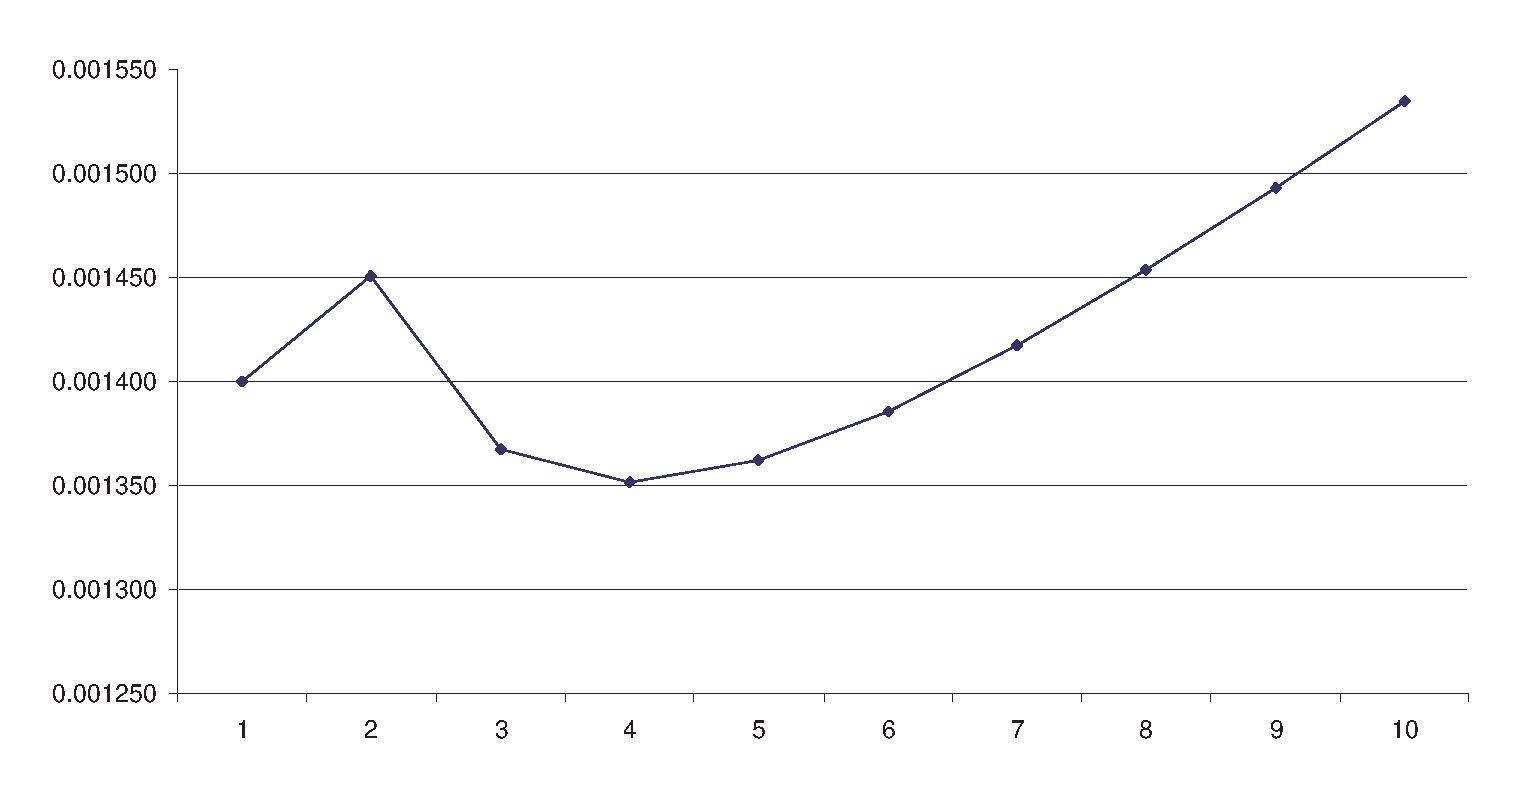
\epsfig{file=psfigures/RedundantCommTimes.eps, width=3.75in}
      \end{center}
\end{enumerate}

\end{enumerate}

\chapter{Sorting}

\begin{enumerate}
\item
Quicksort is not a stable sorting algorithm.

\item {\bf Note: In the first printing of the text there are a couple of typos
      in this exercise. First, $n$ should be 100,000, not 100 million.
      Second, answers should be computed only for $p$ equal to powers of 2:
      1, 2, 4, 8, and 16.}

      This is a difficult problem. I came up with these numbers by actually
      writing an MPI program implementing the first parallel quicksort
      algorithm described in the book, then performing a max-reduction to
      find the maximum partition size. The values in the table represent the
      average over 10 executions of the program.

\begin{enumerate}
\item

\begin{tabular}{|r|r|r|}
\hline
$p$ & {\it Maximum List Size} & Max list size / $\lceil n/p\rceil$ \\
\hline
1  & 100,000 & 1.00 \\
2  &  71,019 & 1.42 \\
4  &  56,428 & 2.26 \\
8  &  39,474 & 3.158 \\
16 &  36,241 & 5.799 \\
\hline
\end{tabular}

\item Parallel execution time is the sum of the computation time and the
      communication time.

      The computation time has two components: partition
      time and quicksort time. At each iteration of the algorithm each
      processor must partition its list of values into two pieces: the piece it
      is keeping and the piece it is passing. This time is about
      $$m(\log p)(0.000000070 {\rm\ sec})$$
      where $m$ is the maximum list size.
      The quicksort time is
      $$(0.000000070 {\rm\ sec})(m \log m - 2.846\log m)$$
      (see Baase and Van Gelder [5] for the expected number of comparisons
      in sequential quicksort).

      The communication time is the time spent exchanging elements.
      We assume sending and receiving happen concurrently.
      We estimate the total communication time by the processor with the
      most elements concurrently sends half of these elements and receives
      half of these elements each iteration.
      The total communication time is
      $$\log p\bigl(0.0002 {\rm\ sec} + (m/2)(4 {\rm\ byte})/(10^7 {\rm\ byte/sec})\bigr)$$

\begin{tabular}{|r|r|r|}
\hline
$p$ & Time (sec) & Speedup \\
\hline
1 &  0.141 & 1.00 \\
2 &  0.116 & 1.21 \\
4 &  0.106 & 1.33 \\
8 &  0.083 & 1.70 \\
16 & 0.086 & 1.64 \\
\hline
\end{tabular}
\end{enumerate}

\item {\bf Note: In the first printing of the text there are a couple of typos
      in this exercise. First, $n$ should be 100,000, not 100 million.
      Second, answers should be computed only for $p$ equal to powers of 2:
      1, 2, 4, 8, and 16.}

      This is a difficult problem. I came up with these numbers by actually
      writing an MPI program implementing the hyperquicksort
      algorithm described in the book, then performing a max-reduction to
      find the maximum partition size. The values in the table represent the
      average over 10 executions of the program.

\begin{enumerate}
\item

\begin{tabular}{|r|r|r|}
\hline
$p$ & {\it Maximum List Size} & Max list size / $\lceil n/p\rceil$ \\
\hline
1  & 100,000 & 1.000 \\
2  &  50,089 & 1.002 \\
4  &  25,151 & 1.006 \\
8  &  12,688 & 1.015 \\
16 &   6,723 & 1.076 \\
\hline
\end{tabular}

\item Parallel execution time is the sum of the computation time and the
      communication time. The execution time formulas are the same as in
      the answer to exercise 14.2. 

\begin{tabular}{|r|r|r|}
\hline
$p$ & Time (sec) & Speedup \\
\hline
1 &  0.1412 & 1.00 \\
2 &  0.0658 & 1.77 \\
4 &  0.0307 & 3.16 \\
8 &  0.0143 & 5.62 \\
16 & 0.0070 & 9.41 \\
\hline
\end{tabular}
\end{enumerate}

\item
We have $n = 10^8$, $\chi = 70$ nanosec, $\lambda = 200\ \mu$sec,
and $\beta = 2.5\times 10^6$ elements/sec.
In the first step each processor sorts $n/p$ elements.
The time required for this is
$$\chi(1.386(n/p)\log(n/p) - 2.846(n/p))$$
The time to gather the pivots is dominated by the message latency:
$$\lambda(\lceil\log p\rceil)$$
Next one process sorts the $p^2$ random samples.
Using quicksort, the estimated time is
$$\chi(1.386(p^2)\log(p^2) - 2.846 p^2$$
Broadcasting $p-1$ pivots to the other processes is dominated by the
message latency:
$$\lambda(\lceil\log p\rceil)$$
Next comes the all-to-all communication step. We assume each process sends
$p-1$ messages and receives $p-1$ messages. These happen concurrently.
The total communication time for this step is
$$(p-1)\lambda + n(p-1)/(p\beta)$$
Finally, each process merges $p$ sorted sublists.
If each step requires $2\log p$ comparisons, the time needed for this
step is
$$2\chi\log p(1.03n/p)$$

The total estimated execution time is
\begin{equation*}
\begin{aligned}
\chi(&1.386((n/p)\log(n/p) + 2p^2\log p) - 2.846((n/p) + p^2)\\
     &+ 2\log p(1.03n/p)) +\\
&\lambda(2\lceil\log p\rceil + (p-1)) + n(p-1)/(p\beta)
\end{aligned}
\end{equation*}

\begin{tabular}{|c|c|c|}
\hline
{\it Processors}&{\it Time (sec)}&{\it Speedup}\\
\hline
1 & 169.9 & 1.00 \\
2 & 88.7 & 1.92 \\
3 & 62.5 & 2.72 \\
4 & 47.2 & 3.60 \\
5 & 40.2 & 4.23 \\
6 & 33.8 & 5.02 \\
7 & 29.3 & 5.79 \\
8 & 26.0 & 6.53 \\
9 & 24.6 & 6.91 \\
10 & 22.4 & 7.58 \\
11 & 20.7 & 8.22 \\
12 & 19.2 & 8.85 \\
13 & 18.0 & 9.46 \\
14 & 16.9 & 10.0 \\
15 & 16.0 & 10.6 \\
16 & 15.2 & 11.2 \\
\hline
\end{tabular}

\item The PSRS algorithm is less disrupted when given a sorted list.

In the first iteration of the hyperquicksort algorithm, the
root process sorts its sublist, then broadcasts the median of its sublist
to the other processes. All processes use this value to divide their lists
into the lower ``half'' and the upper ``half.''
Since the root process has the smallest $n/p$ keys, its estimate of the
median will be very poor.
The root process will send half of its keys to its partner process in the
upper half of the hypercube.
The other processes in the lower half of the hypercube will send all of
their keys to their partner processes in the upper half of the hypercube.
This severe workload imbalance will significantly increase the execution time
of the algorithm.

In contrast, in the PSRS algorithm each process contributes $p$ samples from
its sorted sublist. After sorting the contributed samples, the root process
selects regularly spaced pivot values.
After receiving the pivot values, each process will partition its sorted
sublist into $p$ disjoint pieces.
The largest partition held by process $i$ will be partition $i$.
When each process $i$ keeps its $i$th partition and sends the $j$th
partition to process $j$, relatively few values will be communicated.
Each process should have nearly the same number of elements for the
final mergesort step.

\item
We are going to perform a $p$-way merge of $p$ sorted sublists.
We build a heap from the first element of each sorted sublist.
This takes time $\Theta(p)$.
The root of the heap is the element with the smallest value.
It is the first element of the merged lists.
We remove the heap element and replace it with the next member of
that element's originating sublist.
This can be done in constant time.
We then perform a ``heapify'' operation to restore the heap property.
This step takes $\Theta(\log p)$ time.

Now the root of the heap is the second element of the merged lists.
We repeat the previous delete-replace-heapify procedure.

When an originating sublist is exhausted, we insert a key with
a very large value into the heap, ensuring it will never be chosen 
before an element from one of the other sublists.

We continue until we have deleted from the heap a number of elements
equal to the original total length of all the sublists.
If there were $\Theta(n/p)$ elements total in the $p$ sublists,
the total time required to perform the merge is $\Theta((n/p)\log p)$.

%Skip exercises 14-7 and 14-8
\addtocounter{enumi}{2}

\item
\begin{enumerate}
\item We organize the processes into a binomial tree.
      In the initial $\log p$ steps of the algorithm, each process with
      a list of elements divides its list in half and sends half of its
      list to a partner process.
      After $\log p$ steps, every process has $n/p$ keys.

      Next each process uses sequential mergesort to sorts its sublist.

      Reversing the communication pattern of the first step, during each
      of $\log p$ steps half the processes with a sorted sublist send their
      sublist to another process with a sorted sublist, and the receiving
      processes merges the lists. After $\log p$ of these steps, a single
      process has the entire sorted list.

      This figure illustrates parallel mergesort.

      \begin{center}
      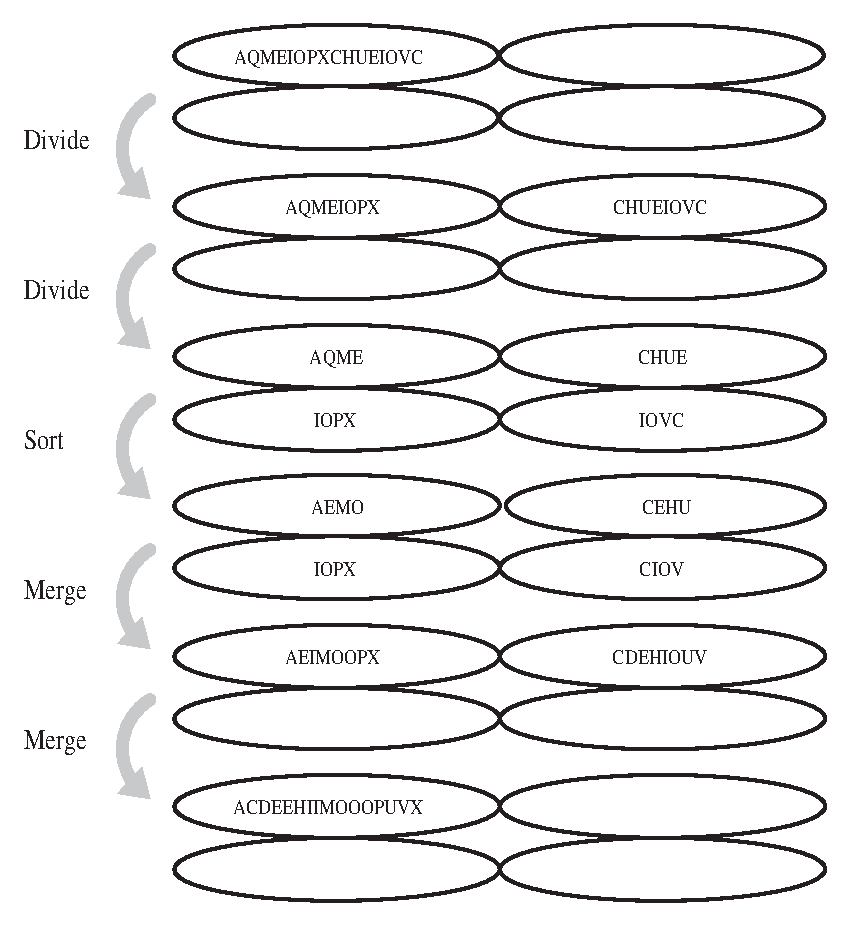
\epsfig{file=psfigures/ParallelMergesort.eps, width=3.75in}
      \end{center}

\item Distributing the unsorted subarrays takes $\log p$ steps.
      In the first step 1 process sends $n/2$ values, in the second
      step 2 processes concurrently send $n/4$ values, and so on.
      Hence the communication complexity of this step is $\Theta(\log p + n)$.
      The time needed for each process to sort its section of $n/p$ values is
      $\Theta((n/p)\log(n/p))$.
      The communication time needed for the merge step
      is $\Theta(\log p + n)$.
      The computation time for the merge step is $\Theta(n)$.
      Hence the overall time complexity of parallel mergesort is
      $\Theta(\log p + n + (n/p)\log(n/p))$.

\item The communication overhead of the algorithm is $p$ times the
      communication complexity, or $\Theta(p(\log p + n))$.
      When $n$ is large the message transmission time dominates the
      message latency, so we'll simplify the communication overhead to
      $\Theta(p\log p)$.
      Hence the isoefficiency function is
      $$n\log n \ge Cp\log p$$
      When we double $p$ we must slightly more than double $n$ in order to
      maintain the same level of efficiency.
      Since $p$ is much smaller than $n$, the algorithm is not perfectly
      scalable.
\end{enumerate}

\item
\begin{enumerate}
\item We divide the interval $[0, k)$ into $p$ buckets (subintervals).
      Each process is responsible for one of these buckets, and every process
      knows the interval handled by each process.
      In step one every process divides its $n/p$ keys into $p$ groups,
      one per bucket.
      In step two an all-to-all communication routes groups of keys to the
      correct processes.
      In step three each process sorts the keys in its bucket using quicksort.
\item Step one has time complexity $\Theta(n/p)$.
      Since $n$ is much larger than $p$, communication time is dominated by
      the time needed to transmit and receive the elements.
      We expect each processor to
      send about $n(p-1)/p$ elements to other processors and receive about
      the same number. Assuming the network has sufficient bandwidth to allow
      each processor to be sending and receiving a message concurrently,
      the time needed for step two is $\Theta(n/p)$.
      Step three has time complexity $\Theta((n/p)\log(n/p))$.
      The overall computational complexity of the parallel bucket sort is
      $\Theta((n/p)\log(n/p))$, and the communication complexity is
      $\Theta(n/p)$.
\item The communication overhead is $p$ times the communication complexity,
      or $\Theta(n)$.
      If there are $p$ buckets, the sequential algorithm requires time
      $\Theta(n)$ to put the values in the buckets and time
      $\Theta((n/p)\log(n/p))$ to sort the elements in each bucket.
      With $p$ buckets, the complexity of the sequential algorithm
      is $\Theta(n\log(n/p))$.
     
      Hence the scalability function is
      $$n\log(n/p) \ge Cn \Rightarrow \log(n/p) \ge C 
                          \Rightarrow n/p \ge 2^C
                          \Rightarrow n \ge 2^Cp$$
      The parallel bucket sort algorithm is not highly scalable.
\end{enumerate}

\end{enumerate}

\chapter{The Fast Fourier Transform}

\begin{enumerate}
\item  \begin{enumerate}
       \item $1 = 1e^{0i}$
       \item $i = 1i^{(\pi/2)i}$
       \item $4 + 3i = 5e^{0.93i}$
       \item $-2 -5i = 5.39e^{4.33i}$
       \item $2 - i = 2.24e^{5.82i}$
       \end{enumerate}

\item Principal 2d root of unity is $-1 = 1e^{\pi i}$.

      Principal 3d root of unity is $-0.5 + 0.87i = 1e^{(2\pi/3)i}$.

      Principal 4th root of unity is $i = 1e^{(\pi/2)i}$.

      Principal 5th root of unity is $0.31 + 0.95i = 1e^{(2\pi/5)i}$.
\item \begin{enumerate}
       \item $(18, -4)$
       \item $(72, -6+6i, -8, -6-6i)$
       \item $(28, -5.83-1.59i, 4+8i, -0.17+4.41i, -8,
              -0.17-4.41i, 4-8i, -5.83+1.59i)$
      \end{enumerate}

\item \begin{enumerate}
       \item $(0.5, 2.5)$
       \item $(1, 2, 3, 4)$
       \item $(1, 1.82, 3.25, 2.03, 3.00, 2.18, -0.25, 0.97)$
      \end{enumerate}

%Skip exercises 15-5 through 15-7
\addtocounter{enumi}{3}

\item Our first parallel quicksort algorithm and hyperquicksort
      exhibit a butterfly communication pattern.
      A butterfly communication pattern is also an appropriate way to perform an
      all-to-all exchange when the communication time is dominated by message
      latency.
      An all-reduce may be performed using a butterfly communication pattern.

\item The sequential versions of both hyperquicksort and the fast Fourier
      transform have time complexity $\Theta(n\log n)$.
      Both parallel algorithms have $\Theta(\log p)$ communication steps,
      each step transmitting $\Theta(n/p)$ values.
      Both parallel algorithms use a butterfly communication pattern that
      enables data starting on any processor to reach any other processor in
      no more than $\log p$ message-passing steps.

\end{enumerate}

\chapter{Combinatorial Search}

\begin{enumerate}

\item The decomposition step cannot be performed in parallel.
      The time needed for decompositions alone is
      $$n + {{n}\over{k}} + {{n}\over{k^2}} + \ldots +
        {{n}\over{k^{\log_k n}}}$$
      Since this sum is $> n$ and $< nk/(k-1)$,
      a good lower bound on the complexity of the parallel algorithm is
      $\Omega(n)$.

\item There are two fundamentally different strategies for limiting the
      number of nodes in the state space tree. I do not know which one is 
      more effective for this problem.

      The first approach is to always fill in the word that would
      cause the most unassigned letters in the puzzle to be given a value.
      By assigning as many letters as possible at each node in the state
      space tree, this strategy aims to minimize the depth of the tree.

      The second approach is to always fill in the word with the fewest
      unassigned letters. In case of a tie, we would choose the longest word
      with the fewest unassigned letters.
      This strategy aims to minimize the number of branches at each node in
      the state space tree.

      The algorithm described in the book represents a middle point between
      the two strategies I have just described.

\item It is unlikely that a simple backtrack search of the state space tree for
      the 8-puzzle will yield a solution, because there is a good probability
      that before the search finds a solution node, it will encounter a node
      whose board position is identical to that of a previously-examined node.
      If this happens, it means that the search has run into a cycle. Assuming
      that the legal moves from a given position are always examined in the
      same order, encountering a cycle guarantees that the search will never
      leave the cycle, and hence a solution will never be found.

      Here are two ways to modify the backtrack search to guarantee it will
      eventually find a solution.

      One way to avoid falling into an infinite cycle is to check
      for cycles every time a move is considered.
      If a move results in a board position already represented by one of
      the ancestor nodes in the state space tree, the move is not made.

      Another way to avoid falling into an infinite cycle 
      is to use iterative deepening; i.e., limiting the search
      to a certain depth.
      First we perform backtrack search to a fixed level $d$.
      If no solution is found, we perform a backtrack search to level $d+1$.
      We continue in this fashion until a solution is found.

\item The lower bound associated with the right node of the root is 7,
      because the eight tiles are out of place by a total of 6 positions
      (using the Manhattan distance calculation), and 1 move has already
      been taken. $6 + 1 = 7$.
      (Tile 5 is 1 position out of place, tile 3 is 2 positions out of place,
      tile 2 is 2 positions out of place, and tile 6 is 1 position out of
      place.)

\item The number of nodes at each level of the state space tree is
      $1, 3, 8, 24,$ $64, \ldots$.
      (Multiply by 3, then multiply by 8/3,
      multiply by 3, multiply by 8/3, etc.)
      A breadth-first search examines all nodes in the first five
      levels of the state space tree, or $1 + 3 + 8 + 24 + 64 = 100$ nodes.
      A breadth-first search also examines all nodes up to and including the
      solution node at the sixth level of the tree.
      There are 96 nodes to the left of the solution node.
      The total number of nodes examined by a breadth-first search of the
      state space tree is 197.

\item In case of a tie, we want to pick the node deeper in the state space
      tree, since its lower bound is based more on definite information
      (the number of constraints added so far), and less on an estimate
      (the lower bound function).

\item The advantage of the proposed best-first branch-and-bound algorithm is
      that it has very little communication overhead. The disadvantage is that
      the workloads among the processes are likely to be highly imbalanced.
      The proposed algorithm is unlikely to achieve higher performance than
      the algorithm presented in the text.

\item If a perfect evaluation function existed, the best move could be found
      simply by evaluating the position resulting from each legal move and
      choosing the position with the highest value.

\item Here is the result of a minimax evaluation of the game tree:
      \begin{center}
      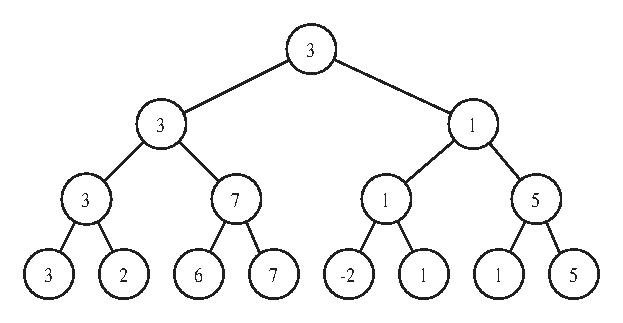
\epsfig{file=psfigures/MinimaxTree.eps, width=3in}
      \end{center}

\item The alpha-beta algorithm prunes the game tree of Figure 16.19 at
      the node labeled B because this is a min node, and the first
      value returned is $-9$. The opponent is able to choose the move.
      Since the opponent is trying to minimize the value, we know that
      the ultimate value of the node is less than or equal to $-9$.
      However, the parent of this node is a max node. Since the player
      already has a move with leading to a position with value $-7$,
      there is no way the player will make a move leading to a position
      with value less than or equal to $-9$, so there is no point in
      continuing the search. The search tree is pruned at this point.

\item Here is the result of an alpha-beta search of the game tree:
      \begin{center}
      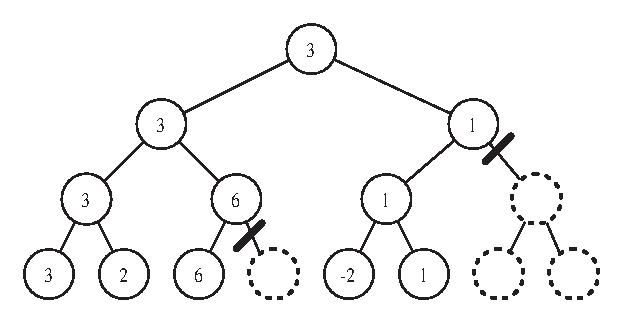
\epsfig{file=psfigures/AlphaBetaTree.eps, width=3in}
      \end{center}

\item Extending the perfectly ordered game tree.

      \begin{center}
      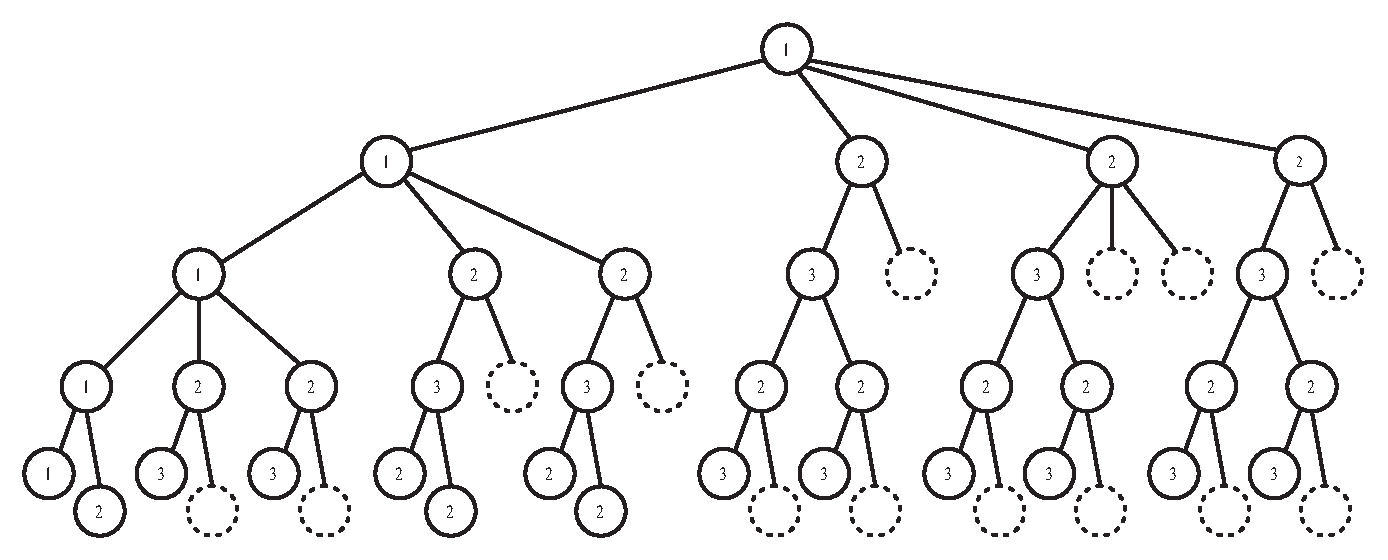
\epsfig{file=psfigures/PerfectlyOrdered.eps, width=4in}
      \end{center}

\item When DTS search reaches a point where there is only a single processor
      allocated to a node, it executes the standard sequential alpha-beta
      search algorithm.
      Hence alpha-beta search is a special case of DTS---the case where
      $p = 1$.

\item Improving the pruning effectiveness of the underlying alpha-beta
      algorithm reduces the speedup achieved by the DTS
      algorithm on a particular application.
      Given a uniform game tree with branching factor $b$, if
      alpha-beta pruning reduces the effective branching factor to $b^x$
      (where $0.5 \le x \le 1$), then speedup achieved by DTS
      with $p$ processors and
      breadth-first allocation will be reduced to $O(p^x)$.
\end{enumerate}

\chapter{Shared-memory Programming}

\begin{enumerate}

\item The two OpenMP function that have closest analogs in MPI functions
      are {\tt omp\_get\_num\_threads} and {\tt omp\_get\_thread\_num}.
      Function {\tt omp\_get\_num\_threads} is similar to
      {\tt MPI\_Comm\_size}. Function {\tt omp\_get\_thread\_num}
      is similar to {\tt MPI\_Comm\_rank}.

\item \begin{enumerate}
      \item {\tt \#pragma omp parallel for}
      \item This code segment is not suitable for execution because the
            control expression of the {\tt for} loop is not in canonical form.
            The number of iterations cannot be determined at loop entry time.
      \item This loop can be executed in parallel assuming there are no
            side effects inside function {\tt foo}. The correct pragma is
            \vskip\baselineskip
            {\tt \#pragma omp parallel for}
      \item This loop can be executed in parallel assuming there are no
            side effects inside function {\tt foo}. The correct pragma is
            \vskip\baselineskip
            {\tt \#pragma omp parallel for}
      \item This loop is not suitable for parallel execution, because it
            contains a {\tt break} statement.
      \item {\tt \#pragma omp parallel for reduction(+:dotp)}
      \item {\tt \#pragma omp parallel for}
      \item This loop is not suitable for parallel execution if {\tt n} is
            greater than or equal to {\tt 2*k}, because in that case there
            is a dependence between the first iteration of the loop
            that assigns a value to {\tt a[k]} and the ({\tt k}+ 1)st
            iteration, that references the value.
      \end{enumerate}

\item Here is a C program segment that computes $\pi$ using a private
      variable and the {\tt critical} pragma.

\begin{verbatim}
double area, pi, subarea, x;
int i, n;

area = 0.0;
#pragma omp parallel private(x, subarea)
{
   subarea = 0.0;
#pragma omp for nowait
   for (i = 0; i < n; i++) {
      x = (i+0.5)/n;
      subarea += 4.0/(1.0 + x*x);
   }
#pragma omp critical
   area += subarea;
}
pi = area / n;
\end{verbatim}

\item Matrices in C are stored in row-major order.
      There is a good chance that the end of one matrix row and the beginning of
      the next matrix row are stored in the same cache block.
      Increasing the chunk size reduces the number of times one thread is
      responsible for one matrix row and another thread is responsible for
      the next matrix row.
      Hence increasing the chunk size reduces the number of times two
      different threads share the same cache block and increases the cache
      hit rate.

\item Here is an example of a simple parallel {\tt for} loop that would
      probably execute faster with an interleaved static scheduling than
      by giving each task a single contiguous chunk of iterations.

\begin{verbatim}
for (i = 0; i < 100000; i++) {
   if (i < 10000) {
      a[i] = (sin(i) + cos(i))*(sin(i) + cos(i));
   } else {
      a[i] = 0.0;
   }
}
\end{verbatim}

\item A good example would be a loop with a small ratio of iterations to
      threads in which the variance in the execution times of each iteration
      is large and cannot be predicted at compile time.

\item Two threads can end up processing the same task if both threads
      are executing function {\tt get\_next\_task} simultaneously and both
      threads execute statement

\begin{verbatim}
answer = (*job_ptr)->task;
\end{verbatim}

      before either thread executes the following statement:

\begin{verbatim}
*job_ptr = (*job_ptr)->next;
\end{verbatim}

      That is why we add the {\tt critical} pragma to ensure the function
      executes atomically.

\item Another OpenMP implementation of the Monte Carlo algorithm to
      compute $\pi$.

\begin{verbatim}
#include <stdlib.h>
#include <stdio.h>

int main (int argc, char *argv[])
{
   int count;            /* Points inside unit circle */
   int i;
   int local_count;      /* This thread's subtotal */
   int samples;          /* Points to generate */
   unsigned short xi[3]; /* Random number seed */
   double x, y;          /* Coordinates of point */

   samples = atoi(argv[1]);
   omp_set_num_threads (atoi(argv[2]));
   count = 0;
#pragma omp parallel private(xi,x,y,local_count)
   {
   local_count = 0;
   xi[0] = 1;
   xi[1] = 1;
   xi[2] = omp_get_thread_num();
#pragma omp for nowait
   for (i = 0; i < samples; i++) {
      x = erand48(xi);
      y = erand48(xi);
      if (x*x + y*y <= 1.0) local_count++;
   }
#pragma omp critical
   count += local_count;
   }
   printf ("Estimate of pi: %7.5f\n", 4.0*count/samples);
}
\end{verbatim}

\item Code segment from Winograd's matrix multiplication algorithm,
      augmented with OpenMP directives.

\begin{verbatim}
#pragma omp parallel
{
    #pragma omp for private(j) nowait
    for (i = 0; i < m; i++) {
       rowterm[i] = 0.0;
       for (j = 0; j < p; j++)
       rowterm[i] += a[i][2*j] * a[i][2*j+1];
    }
    #pragma omp for private(j) nowait
    for (i = 0; i < q; i++) {
       colterm[i] = 0.0;
       for (j = 0; j < p; j++)
          colterm[i] += b[2*j][i] * b[2*j+1][i]; 
    }
}
}
\end{verbatim}

      Alternatively, we could have
      used the {\tt sections} pragma to enable both {\tt for} loops indexed
      by {\tt i} to execute concurrently.

\begin{verbatim}
#pragma omp parallel
{
    #pragma omp sections
    {
    #pragma omp section
    for (i = 0; i < m; i++) {
       rowterm[i] = 0.0;
       for (j = 0; j < p; j++)
       rowterm[i] += a[i][2*j] * a[i][2*j+1];
    }
    #pragma omp section
    for (i = 0; i < q; i++) {
       colterm[i] = 0.0;
       for (j = 0; j < p; j++)
          colterm[i] += b[2*j][i] * b[2*j+1][i]; 
    }
    }
}
\end{verbatim}

      Some compilers may
      allow both parallelizations.  However, the Sun
      compiler does not allow a {\tt for} pragma to be nested inside a
      {\tt sections} pragma.

\end{enumerate}

\chapter{Combining MPI and OpenMP}

\begin{enumerate}
\item 

We consider the suitability of each of the program's functions for
parallelization using threads.

{\tt main}---The function contains no {\tt for} loops.
It has no large blocks of code that
two or more threads could execute concurrently. It is not suitable for
parallelization using threads.

{\tt manager}---The only {\tt for} loop in the function is the one that
copies the document profile vector from {\tt buffer} to
{\tt vector[assigned[src]]}. If the vector is long enough, this step could
benefit from execution by concurrent threads. Before doing this,
however, the {\tt for} loop should be changed to a {\tt memcpy} operation.
There are no large blocks of code that two or more threads could execute
concurrently.

{\tt worker}---The function contains no {\tt for} loops in canonical form.
It has no large blocks of code that two or more threads could execute
concurrently. It is not suitable for parallelization using threads.

{\tt build\_2d\_array}---This function takes little time to execute.

{\tt get\_names}---This function searches a directory structure for names
of documents to be profiled. The speed of this search could be improved by
dividing subdirectories among threads.

{\tt write\_profiles}---This function writes profile vectors to a single
file. It is not suitable for concurrent execution.

{\tt build\_hash\_table}---This function initializes an array of pointers
and takes little time to execute.

{\tt make\_profile}---This function builds a profile vector from the words
in a document. We can imagine most of the program's execution time is spent
inside this function. Assuming the profile vector for an entire document can
be created from profile vectors of the document's pieces, this function is
a good candidate for parallelization via threads.

{\tt read\_dictionary}---This function reads words from a single file.
It is not a good candidate for parallelization.

From our analysis it appears the functions that are the
best candidates for parallelization with OpenMP pragmas are
{\tt make\_profile} and {\tt get\_names}.

\item The book describes three situations in which mixed MPI/OpenMP programs
      can outperform MPI-only programs.

      The first situation is when the mixed MPI/OpenMP program has lower
      communication overhead than the MPI-only program.
      Monte Carlo methods typically have very little communication among the
      processes. Hence this situation probably does not hold.

      The second situation is when it is practical to parallelize some
      portions of the computation via lighter weight threads, but not via
      heavier weight processes.
      In the case of a Monte Carlo program, the entire computation is
      completely parallelizable---every process is executing the simulation
      with a different stream of random numbers.
      Hence this situation probably does not hold.

      The third situation is when some MPI processes are idle when others
      are busy, due to message-passing or other I/O operations. This is 
      most likely not the case for Monte Carlo simulations.

      The conclusion is that there are poor prospects for significantly
      improving the performance of the Monte Carlo methods by converting
      them into MPI/OpenMP programs.

\end{enumerate}
\end{document}               % End of document.
